%%%%%%%%%%%%%%%%%%%%%%%%%%%%%%%%%%%%%%%%%
% Beamer Presentation
% LaTeX Template
% Version 1.0 (10/11/12)
%
% This template has been downloaded from:
% http://www.LaTeXTemplates.com
%
% License:
% CC BY-NC-SA 3.0 (http://creativecommons.org/licenses/by-nc-sa/3.0/)
%
%%%%%%%%%%%%%%%%%%%%%%%%%%%%%%%%%%%%%%%%%

%----------------------------------------------------------------------------------------
%	PACKAGES AND THEMES
%----------------------------------------------------------------------------------------

\documentclass{beamer}

\mode<presentation> {

% The Beamer class comes with a number of default slide themes
% which change the colors and layouts of slides. Below this is a list
% of all the themes, uncomment each in turn to see what they look like.
\usetheme{AnnArbor}
%\usetheme{default}
%\usetheme{AnnArbor}
%\usetheme{Antibes}
%\usetheme{Bergen}
%\usetheme{Berkeley}
%\usetheme{Berlin}
%\usetheme{Boadilla}
%\usetheme{CambridgeUS}
%\usetheme{Copenhagen}
%\usetheme{Darmstadt}
%\usetheme{Dresden}
%\usetheme{Frankfurt}
%\usetheme{Goettingen}
%\usetheme{Hannover}
%\usetheme{Ilmenau}
%\usetheme{JuanLesPins}
%\usetheme{Luebeck}
%\usetheme{Madrid}
%\usetheme{Malmoe}
%\usetheme{Marburg}
%\usetheme{Montpellier}
%\usetheme{PaloAlto}
%\usetheme{Pittsburgh}
%\usetheme{Rochester}
%\usetheme{Singapore}
%\usetheme{Szeged}
%\usetheme{Warsaw}

% As well as themes, the Beamer class has a number of color themes
% for any slide theme. Uncomment each of these in turn to see how it
% changes the colors of your current slide theme.

%\usecolortheme{albatross}
%\usecolortheme{beaver}
%\usecolortheme{beetle}
%\usecolortheme{crane}
%\usecolortheme{dolphin}
%\usecolortheme{dove}
%\usecolortheme{fly}
%\usecolortheme{lily}
%\usecolortheme{orchid}
%\usecolortheme{rose}
%\usecolortheme{seagull}
%\usecolortheme{seahorse}
%\usecolortheme{whale}
%\usecolortheme{wolverine}

%\setbeamertemplate{footline} % To remove the footer line in all slides uncomment this line
%\setbeamertemplate{footline}[page number] % To replace the footer line in all slides with a simple slide count uncomment this line

%\setbeamertemplate{navigation symbols}{} % To remove the navigation symbols from the bottom of all slides uncomment this line
}
\graphicspath{{./figures/}}

\usepackage{graphicx} % Allows including images
\usepackage{booktabs} % Allows the use of \toprule, \midrule and \bottomrule in tables
\usepackage{amsmath,bm, amsthm, mathtools}
\usepackage{lineno,hyperref,amssymb,graphicx,float,subcaption}
\usepackage{amsmath,bm, amsthm, mathtools}
\usepackage[ruled,vlined]{algorithm2e}
\SetKwComment{Comment}{$\triangleright$\ }{}
\usepackage{color}
\usepackage{geometry}
\usepackage{pdflscape}
\modulolinenumbers[5]

\theoremstyle{remark}
%\newdefinition{remark}{Remark}
%\newtheorem{prop}{Proposition}
%\theoremstyle{definition}
%\newtheorem{definition}{Definition}[section]

\newcommand{\etal}{\textit{et al}.}
\newcommand{\ie}{\textit{i}.\textit{e}., }
\newcommand{\eg}{\textit{e}.\textit{g}. }
\newcommand{\viscosity}{\nu}
\newcommand{\dt}{\Delta t}
\newcommand{\mc}{\mathcal}
\def\floor#1{\lfloor #1 \rfloor}
\newcommand{\norm}[1]{\left\lVert #1 \right\rVert}
\DeclareMathOperator*{\argmax}{arg\,max}
\DeclareMathOperator*{\argmin}{arg\,min}
\def\Eqref#1{Eq.~(\ref{#1})}


%----------------------------------------------------------------------------------------
%	TITLE PAGE
%----------------------------------------------------------------------------------------

\title[CVRG SUMMER 2021 PDE with NNs]{Modeling the Dynamics of PDE Systems with
Physics-Constrained Deep Auto-Regressive Networks} % The short title appears at the bottom of every slide, the full title is only on the title page

\author{Nicholas Genevaa, Nicholas Zabaras} % Your name
\institute[UND] % Your institution as it will appear on the bottom of every slide, may be shorthand to save space
{
University of Notre Dame\\ % Your institution for the title page
\medskip
\textit{ngeneva@nd.edu} % Your email address
\textit{nzabaras@nd.edu}
\footnote{Code available at: \href{https://github.com/cics-nd/ar-pde-cnn}{https://github.com/cics-nd/ar-pde-cnn}.}
}


% \date{\today} % Date, can be changed to a custom date

\begin{document}

\begin{frame}
\titlepage % Print the title page as the first slide
\end{frame}

\begin{frame}
\frametitle{Overview} % Table of contents slide, comment this block out to remove it
\tableofcontents % Throughout your presentation, if you choose to use \section{} and \subsection{} commands, these will automatically be printed on this slide as an overview of your presentation
\end{frame}

%----------------------------------------------------------------------------------------
%	PRESENTATION SLIDES
%----------------------------------------------------------------------------------------

%------------------------------------------------
\section{Introduction} % Sections can be created in order to organize your presentation into discrete blocks, all sections and subsections are automatically printed in the table of contents as an overview of the talk
%------------------------------------------------

%\subsection{Claims} % A subsection can be created just before a set of slides with a common theme to further break down your presentation into chunks
\begin{frame}
\frametitle{Overview}
\begin{itemize}
\item An AutoRegressive
\item Dense Encoder-Decoder
\item CNN
\item Non-linear dynamic systems
\item Without Training (training data)
\item No more Computational Cost than Standard Numerical Methods

\end{itemize}
\end{frame}

\section{Problem Definition}
%------------------------------------------------

\begin{frame}
\frametitle{General PDE Equation}

We are interested in surrogate models of non-linear dynamical systems in a space-time domain.

\begin{equation}
    \begin{gathered}
    \bm{u}(\bm{x},t)_{t}+F\left(\bm{x}, \bm{u}\left(\bm{x},t\right)\right) = 0, \quad  \bm{x}\in\Omega, \: t\in[0,T],\\ 
    \mathcal{B}(\bm{u}) = b\left(\bm{x},t\right), \quad \bm{x}\in\Gamma,\\
    \bm{u}(\bm{x},0) \sim p\left(\bm{u}(\bm{x},0)\right),
    \end{gathered}
    \label{eq:general-pde}
\end{equation}

\begin{equation}
    \bm{u}^{n+1} = f\left(\bm{\chi}^{n+1}, \textbf{w}\right), \quad \bm{\chi}^{n+1} \equiv \left\{\bm{u}^{n}, \bm{u}^{n-1}, \ldots, \bm{u}^{n-k} \right\},
    \label{eq:time-integration}
\end{equation}

\end{frame}

\begin{frame}
\frametitle{Time Equation and Recursion}
\begin{align}
\begin{split}
    \bm{u}^{1} = f\left(\bm{\chi}^{1}, \textbf{w}\right), &\quad \bm{\chi}^{1} = \left\{\bm{u}_{0}, \bm{u}_{0}, \bm{u}_{0}, \ldots, \bm{u}_{0} \right\},\\
    \bm{u}^{2} = f\left(\bm{\chi}^{2}, \textbf{w}\right), &\quad \bm{\chi}^{2} = \left\{\bm{u}^{1}, \bm{u}_{0}, \bm{u}_{0}, \ldots, \bm{u}_{0} \right\},\\
    \bm{u}^{3} = f\left(\bm{\chi}^{3}, \textbf{w}\right), &\quad \bm{\chi}^{3} = \left\{\bm{u}^{2}, \bm{u}^{1}, \bm{u}_{0}, \ldots, \bm{u}_{0} \right\},\\
    \ldots \\
    \bm{u}^{N} = f\left(\bm{\chi}^{N}, \textbf{w}\right), &\quad \bm{\chi}^{N} = \left\{\bm{u}^{N-1}, \bm{u}^{N-2}, \ldots, \bm{u}^{N-1-k} \right\},
    \label{eq:time-int}
\end{split}
\end{align}

\begin{equation}
    \bm{u}^{n+1} = f\left(\left\{ f\left(\bm{\chi}^{n}, \textbf{w}\right), f\left(\bm{\chi}^{n-1}, \textbf{w}\right), \ldots, f\left(\bm{\chi}^{n-k}, \textbf{w}\right) \right\}, \textbf{w}\right),
    \label{eq:recursive}
\end{equation}

\end{frame}

\begin{frame}
\frametitle{Loss Functions}
\begin{equation}
    \argmin_{\textbf{w}} \norm{f\left(\bm{\chi}^{n+1}, \textbf{w}\right) -  T_{\Delta t}\left(\bm{\mathcal{U}}^{n+1}, F_{\Delta x}(\cdot)\right)}^{2}_{2},
    \label{eq:general-loss}
\end{equation}
\end{frame}

\subsection{Surrogate Modeling of Dynamical Systems}

\begin{frame}
\frametitle{Deterministic Surrogate Model}

We pose the following definition for this surrogate model:
\theoremstyle{definition}
\begin{definition}{(Deterministic Surrogate Model)}
For a transient PDE system with specified boundary conditions, as in~\Eqref{eq:general-pde}, and a finite set of initial conditions $\mathcal{S}=\left\{\bm{u}_{0,i}\right\}_{i=1}^{M}$, $\bm{u}_{0,i} \sim p\left(\bm{u}_{0}\right)$, train a surrogate to predict the dynamical response $\bm{y}=\hat{f}\left(\bm{u}_{0}^{*}, \textbf{w}\right)$ for any initial condition, $\bm{u}_{0}^{*} \sim p\left(\bm{u}_{0}\right)$, such that the predicted response is the solution of the governing PDEs for the respective initial state.
\end{definition}

\end{frame}

\begin{frame}
\frametitle{Probabilistic Surrogate Model}
\theoremstyle{definition}
\begin{definition}{(Probabilistic Surrogate Model)}
    For a transient PDE system with specified boundary conditions, such as~\Eqref{eq:general-pde}, and a finite set of initial conditions $\mathcal{S}=\left\{\bm{u}_{0,i}\right\}_{i=1}^{M}$, $\bm{u}_{0,i} \sim p\left(\bm{u}_{0}\right)$, train a surrogate to predict the dynamical response density, $p\left(\bm{y}| \bm{u}_{0}^{*}, \mathcal{S}\right)$, such that the samples drawn from the predictive distribution satisfy the governing PDEs for the respective initial state.
\end{definition}
\end{frame}

\section{Auto-regressive Dense Encoder-Decoder}

\subsection{AR-DenseED}


\begin{frame}
\frametitle{AR-DenseED Schematic}
\begin{figure}[H]
    \centering
    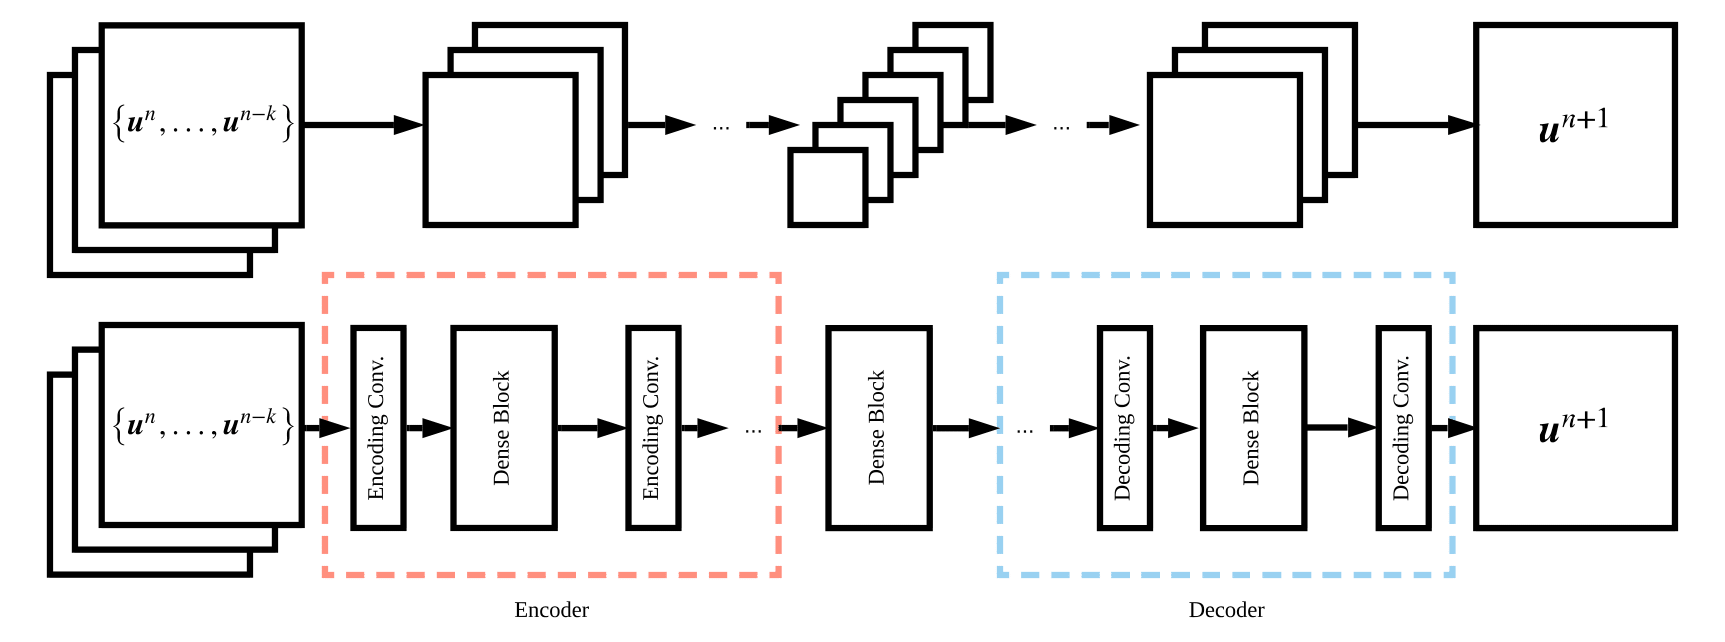
\includegraphics[trim={0 0.25cm 0 0},clip, width=0.8\textwidth]{Fig01.png}
    \caption{Schematic of the auto-regressive dense encoder-decoder.     
    The top shows the dimensionality of the data in the network, the bottom shows the model architecture.
    Using encoding convolutions lowers the dimensionality of the input feature map, while decoding convolutions increase the dimensionality.
    The encoding-decoding process is interleaved with dense blocks that contain multiple densely connected layers in which the dimensionality of the feature maps is held constant.}
    \label{fig:ar-denseED}
\end{figure}
\end{frame}

\begin{frame}
\frametitle{AR-DenseED Training}
\begin{figure}[H]
    \centering
    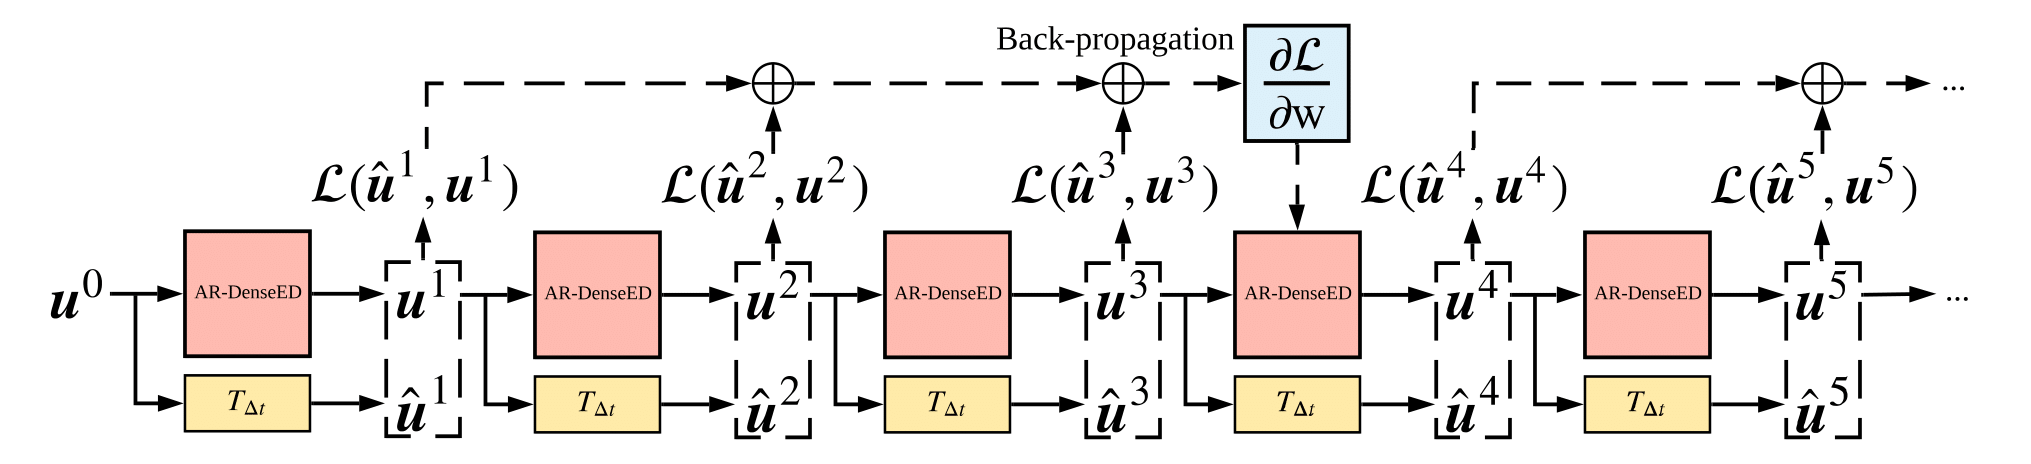
\includegraphics[width=0.9\textwidth]{Fig03.png}
    \caption{Multi-time-step back-propagation of the AR-DenseED where $\textbf{w}$ are the model's learnable weights, $\bm{u}^{n}$ is the model's prediction at time-step $n$, $\hat{\bm{u}}^{n}$ is the target value calculated using the numerical time-integrator $T_{\Delta t}$, and $\mathcal{L}$ is the physics-constrained loss at a single time-step.
    In this example, the computational graph evaluated during back-propagation spans all three predictions resulting in each contributing to the gradient descent update.}
    \label{fig:multi-backprop}
\end{figure}

\end{frame}

\begin{frame}
\frametitle{Algorithm 1: AR-DenseED Prediction}
\begin{figure}
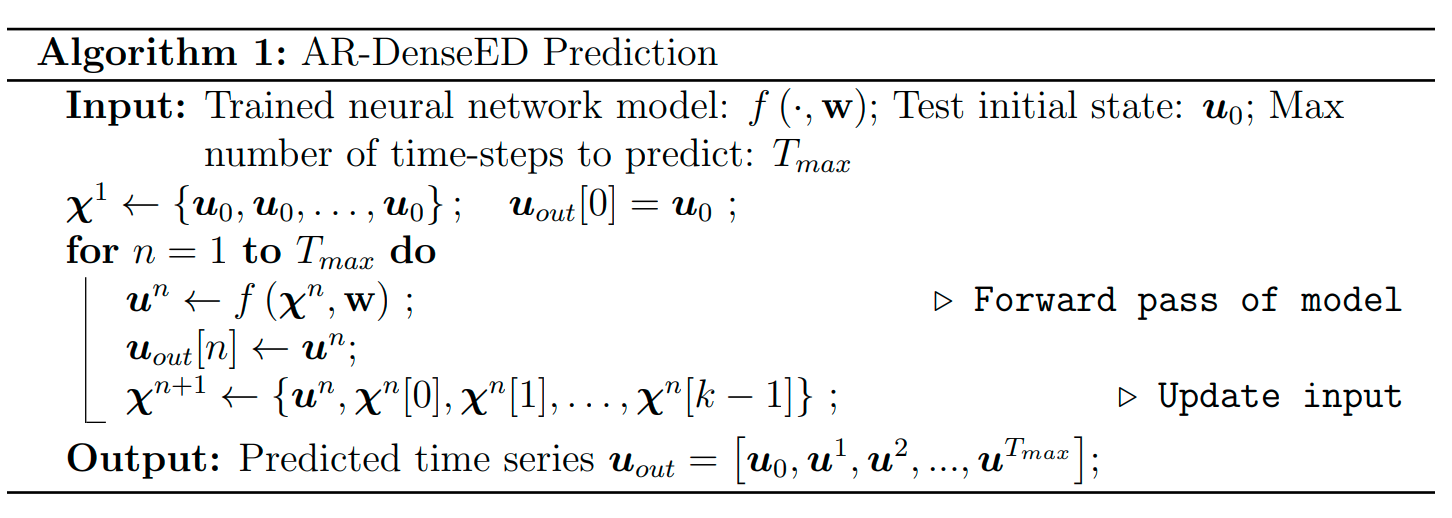
\includegraphics[width=0.9\textwidth]{alg1.png}
\end{figure}
\end{frame}

\begin{frame}
\frametitle{Algorithm 2: Training AR-DenseED}
\begin{figure}
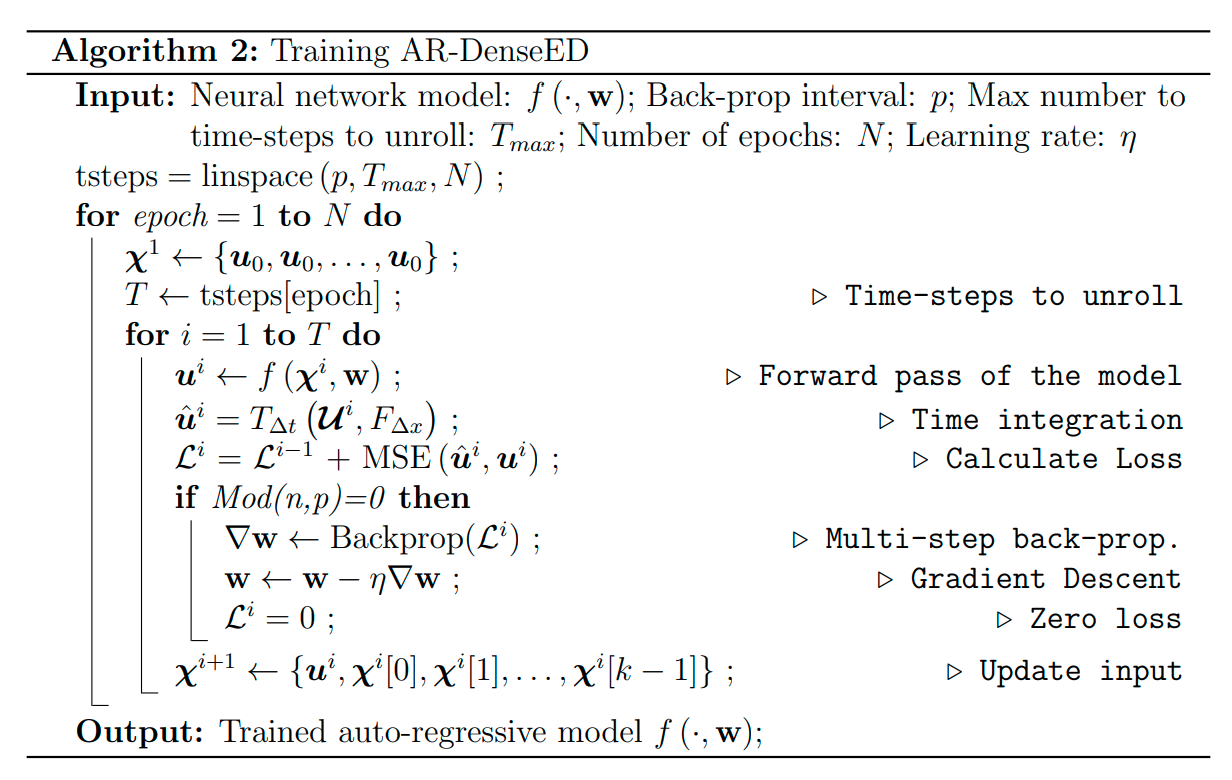
\includegraphics[width=0.9\textwidth]{alg2.png}
\end{figure}

\end{frame}

\subsection{Bayesian AR-DenseED}

\begin{frame}
\frametitle{Bayesian AR-DenseED - Motivation}
In this work, we propose a novel Bayesian framework for physics-constrained models that allow for interpretable uncertainty measures to be produced in the absence of training data.

Account for two major uncertainity components

\begin{itemize}
\item{\textit{aleotoric} which quantifies noise in the observations}
\item{\textit{epistemic} which quantifies inherent uncertainty in the model}
\end{itemize}

However, The numerical time-integrator in the Loss Function introduces truncation error:
\begin{equation}
    \bm{u}_{i}^{n+1} = T_{\Delta t}\left(\bm{\mathcal{U}}^{n+1}, F_{\Delta x}\right) + E_{\Delta t} + E_{\Delta x},
\end{equation}
where $E_{\Delta t}$ and $E_{\Delta x}$ denote the error associated with the discretization of the temporal and spatial derivatives, respectively.

\end{frame}

\begin{frame}
\frametitle{Bayesian AR-DenseED - Posterior Formulation}
We account for the potential discretization error that may arise from $T_{\Delta t}$ through additive output-wise noise, $\epsilon$, for a single arbitrary time-step:
\begin{equation}
    \hat{\bm{u}}^{i} = f\left(\bm{\chi}^{i},\textbf{w}\right) + \epsilon, \quad p\left(\epsilon\right)= \mathcal{N}\left(\epsilon\,|0,\beta^{-1}\bm{I}_{d}\right),
\end{equation}
where for mathematical convenience, we represent the discretized state variables $\bm{u}$ and $\hat{\bm{u}}$ as vectors in $\mathbb{R}^{d}$.
$\bm{I}_{d}$ denotes the identity matrix in $\mathbb{R}^{d\times d}$.
The additive noise is taken as Gaussian with a \textit{learnable} precision $\beta$.
Thus the likelihood for a single time-step, $i$, becomes the following:
\begin{align}
   p\left(\hat{\bm{u}}^{i}|\bm{\chi}^{i},\textbf{w}, \beta\right)&=\mathcal{N}\left(\hat{\bm{u}}^{i}|f\left(\bm{\chi}^{i},\textbf{w}\right), \beta^{-1}\bm{I}_{d}\right), \nonumber\\
   &=\mathcal{N}\left(T_{\Delta t}\left(\bm{\mathcal{U}}^{i}, F_{\Delta x}\right)|f\left(\bm{\chi}^{i},\textbf{w}\right), \beta^{-1}\bm{I}_{d}\right).
\end{align}
Both the inputs to the model $\bm{\chi}^{i}$  and time-integrator $\bm{\mathcal{U}}^{i}$ are found from the deterministic evolution of the model until time-step $i$.
\end{frame}

\begin{frame}
\frametitle{Bayesian AR-DenseED - Posterior Formulation}
Under the Markov assumption, we can formulate the likelihood of an entire time-sequence as the product of individual steps:
\begin{align}
    p\left(\hat{\bm{u}}^{N}, \ldots, \hat{\bm{u}}^{1}|\bm{u}_{0},\textbf{w}, \beta\right) &= \prod_{i=1}^{N}p\left(\hat{\bm{u}}^{i}| \bm{\chi}^{i},\textbf{w}, \beta\right), \nonumber \\
    &= \prod_{i=1}^{N}\mathcal{N}\left(T_{\Delta t}\left(\bm{\mathcal{U}}^{i}, F_{\Delta x}\right)| f\left(\bm{\chi}^{i},\textbf{w}\right), \beta^{-1}\bm{I}_{d}\right). \label{eq:likelihood}
\end{align}
\end{frame}


\begin{frame}
\frametitle{Bayesian AR-DenseED - Posterior Formulation}
A gamma prior is assigned to the noise precision $\beta$:
\begin{equation}
    p(\beta)=\Gamma\left(\beta|a_{1},b_{1}\right),
\end{equation}
where $a_{1}$ and $b_{1}$ are the shape and rate parameters, respectively.
The hyper-parameters of the $\beta$ prior are set based on the \textit{a priori} estimate of the magnitude of the discretization error of $T_{\Delta t}$ and  $F_{\Delta x}$.

\end{frame}

\begin{frame}
\frametitle{Bayesian AR-DenseED - Posterior Formulation}
Given an arbitrary system, we can express the temporal truncation error in the following formula which is standard in Richardson extrapolation~\cite{richardson1927viii}:
 \begin{align}
    \hat{\bm{u}}^{i} &= T_{\Delta t}\left(\bm{\mathcal{U}}^{i}, F_{\Delta x}\right) + c_{0}\left(\Delta t\right)^{k_{0}} + c_{1}\left(\Delta t\right)^{k_{1}} + c_{2}\left(\Delta t\right)^{k_{2}} + \dots \nonumber \\
     &= T_{\Delta t}\left(\bm{\mathcal{U}}^{i}, F_{\Delta x}\right) + c_{0}\left(\Delta t\right)^{k_{0}} + \mathcal{O}\left(\left(\Delta t\right)^{k_{1}}\right),\label{eq:richard0}
\end{align}
where $c_{i}$ are unknown constants, and $k_{i}$ are constants denoting the ``order'' of the error term such that $\left(\Delta t\right)^{k_{i}} > \left(\Delta t\right)^{k_{i+1}}$.
Under the assumption that higher-order terms are negligible, we take the expected value of our prior to be $\mathbb{E}\left(\beta^{-1}\right)=c_{0}\left(\Delta t\right)^{k_{0}}$. 
Additionally this prior is given a large variance to reduce its strength.
\end{frame}

\begin{frame}
\frametitle{Bayesian AR-DenseED - Posterior Formulation}
As is standard for Bayesian neural networks, the network's $K$ learnable parameters, $\textbf{w}$, are treated as random variables.
Due to the large number of weights in our model, we propose a fully factorizable zero mean Gaussian with a Gamma-distributed precision scalar $\alpha$:
\begin{equation}
    p\left(\mathbf{w}|\alpha\right)=\mathcal{N}\left(\mathbf{w}|0, \alpha^{-1}\bm{I}_{K}\right), \quad p\left(\alpha\right) = Gamma\left(\alpha|a_{0},b_{0}\right),
\end{equation}
where the rate parameter $a_{0}$ and the shape parameter $b_{0}$ are $0.5$ and $10$,  respectively.
This results in a prior with a Student's $\mathcal{T}$ density centered at zero that has a wider support region than a standard Gaussian.

\end{frame}

\begin{frame}
\frametitle{Bayesian AR-DenseED - Posterior Formulation}
For a batch of $M$ i.i.d. training scenarios, $\mathcal{S}=\left\{\bm{u}_{0,i}\right\}_{i=1}^{M}$, the joint posterior of the network discounts the prior as follows:
\begin{align}
    p\left(\textbf{w},\beta|\mathcal{S}\right) & \sim \prod^{M}_{j=1} p\left(\hat{\bm{u}}_{j}^{N}, \ldots, \hat{\bm{u}}_{j}^{1}|\bm{u}_{0,j},\textbf{w},\beta\right)p\left(\textbf{w}\right)p\left(\beta\right),  \nonumber \\ 
    & \sim \prod^{M}_{j=1}\prod_{i=1}^{N}\left[p\left(\hat{\bm{u}}_{j}^{i}|\bm{\chi}_{j}^{i},\textbf{w},\beta\right)\right]p\left(\textbf{w}|\alpha\right)p\left(\alpha|a_{0},b_{0}\right)p\left(\beta|a_{1},b_{1}\right),  \nonumber\\
    & \begin{multlined}\sim \prod^{M}_{j=1}\prod_{i=1}^{N} \left[\mathcal{N}\left(T_{\Delta t}\left(\bm{\mathcal{U}}_{j}^{i}, F_{\Delta x}\right)| f\left(\bm{\chi}_{j}^{i},\textbf{w}\right), \beta^{-1}\bm{I}_{d}\right)\right] \mathcal{N}\left(\mathbf{w}|0, \alpha^{-1}\bm{I}_{K}\right)\\
    \qquad \Gamma\left(\alpha| a_{0}, b_{0}\right) \Gamma\left(\beta|a_{1},b_{1}\right).
    \end{multlined}
    \label{eq:posterior-form}
\end{align}
\end{frame}

\begin{frame}
\frametitle{Maximum A posteriori Probability (MAP)}
For sampling the posterior of BAR-DenseED, we will use a recently proposed Stochastic Weight Averaging Gaussian (SWAG)~\cite{maddox2019simple}.
SWAG approximates the posterior in two phases:
\begin{enumerate}
    \item We optimize the model using the ADAM~\cite{kingma2014adam}, an extension of SGD, with exponential learning rate decay.
    \item Once the model has been trained, Stochastic Gradient Descent (SGD) is ran again at a constant learning rate.
    During this process, samples of the model's parameters are collected.
    The core idea is to use SGD to explore the local support region of the MAP estimate.
\end{enumerate}
\end{frame}

\begin{frame}
\frametitle{BAR-DenseED Posterior with SWAG}
A Gaussian distribution with $S$ samples of the model's parameters:
\begin{align}
    &p(\bm{\theta}|\mathcal{S}) \sim \mathcal{N}\left(\bm{\theta}_{SWA}, \bm{\Sigma}_{SWA}\right), \quad \bm{\theta} \equiv \left\{\textbf{w}, ln(\beta)\right\},\\
    &\bm{\theta}_{SWA}=\frac{1}{S}\sum_{i=1}^{S}\bm{\theta}_{i}, \quad \bm{\Sigma}_{SWA}=\frac{1}{2}\left(\bm{\Sigma}_{Diag}+\bm{\Sigma}_{lr}\right),\\
    &\bar{\bm{\theta}}^{2}=\frac{1}{S}\sum_{i=1}^{S}\bm{\theta}^{2}_{i}, \quad \bm{\Sigma}_{Diag} = \textrm{Diag}\left(\bar{\bm{\theta}^{2}}-\bm{\theta}_{SWA}^{2}\right),\\
    &\bm{\Sigma}_{lr}=\frac{1}{K-1}\bm{D}\bm{D}^{T}, \quad \bm{D}_{i} = \left(\bm{\theta}_{i}-\bm{\theta}_{SWA}\right),
\end{align}

where $\bm{\theta}_{i}$ are the model parameters at epoch $i$, and 

$\bm{D} \in \mathbb{R}^{K\times H}$ is a deviation matrix consisting of the $H$ most recent parameter samples forming a low-rank approximation.

$\bm{D}_{i} \in \mathbb{R}^{K}$ is a column of this deviation matrix.
\end{frame}

\begin{frame}
\frametitle{Approximating the BAR-DenseED Posterior with SWAG}
\begin{figure}
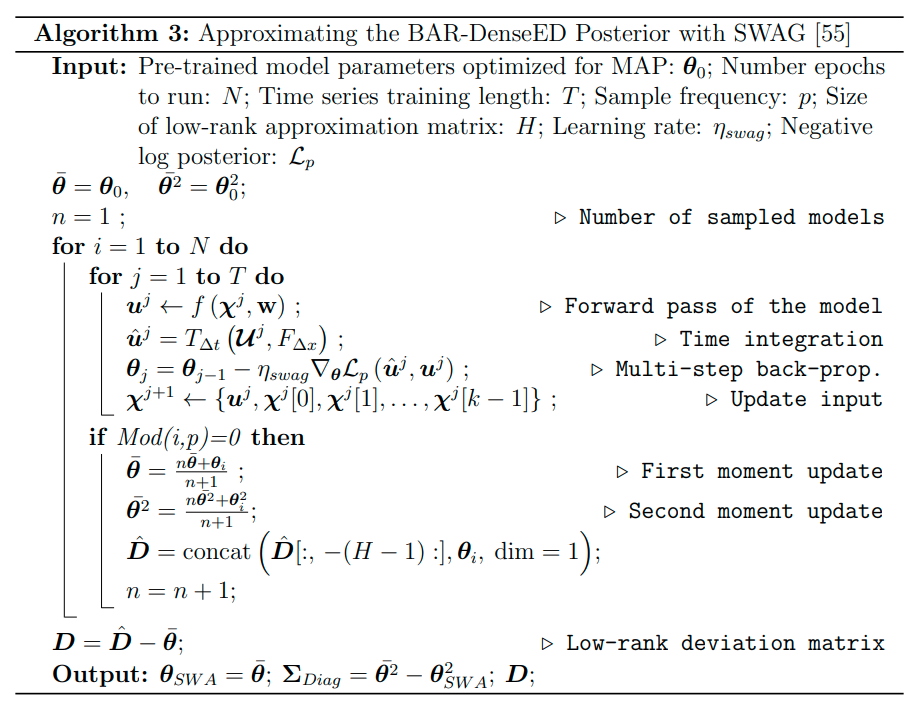
\includegraphics[width=0.8\textwidth]{./figures/alg3.png}
\end{figure}
\end{frame}

\begin{frame}
\frametitle{Predictive Statistics}
We will approximate the marginalization of the model parameters, often referred to as Bayesian model averaging, using Monte Carlo with $P$ parameter samples:
\begin{align}
   p\left(\hat{\bm{u}}^{*}|\bm{\chi}^{*},\mathcal{S}\right)&=\int p\left(\hat{\bm{u}}^{*}|f\left(\bm{\chi}^{*},\textbf{w}\right) ,\beta^{-1}\bm{I}\right)p\left(\textbf{w},\beta|\mathcal{S}\right)d\textbf{w}d\beta,  \nonumber \\
    &\approx \frac{1}{P}\sum_{i=1}^{P}p\left(\hat{\bm{u}}^{*}|f\left(\bm{\chi}^{*},\textbf{w}_{i}\right) ,\beta_{i}^{-1}\bm{I}\right), \quad \left\{\textbf{w}_{i},\beta_{i}\right\} \sim p\left(\bm{\theta}|\mathcal{S}\right),
\end{align}
where $\bm{\chi}^{*}$ and $\hat{\bm{u}}^{*}$ are the predictive inputs and outputs, respectively.
\end{frame}

\begin{frame}
\frametitle{Predictive Statistics}
The posterior, $p(\bm{\theta}|\mathcal{S}) \equiv p(\textbf{w}, ln(\beta)|\mathcal{S})$, has been approximate by SWAG and is easily sampled from.
The predictive expectation can be obtained as follows:
\begin{align}
    \mathbb{E}\left[\hat{\bm{u}}^{*}|\bm{\chi}^{*},\mathcal{S}\right]&=\mathbb{E}_{p\left(\bm{\theta}|\mathcal{S}\right)}\left[\mathbb{E}\left(\hat{\bm{u}}^{*}|\bm{\chi}^{*},\textbf{w},\beta\right)\right],  \nonumber  \\
    &=\mathbb{E}_{p\left(\textbf{w}|\mathcal{S}\right)}\left[f\left(\bm{\chi}^{*},\textbf{w}\right)\right] \approx \frac{1}{P}\sum_{i=1}^{P}f\left(\bm{\chi}^{*},\textbf{w}_{i}\right),
    \label{eq:predictive-mean}
\end{align}
where the additive output noise is not present due to its zero-mean Gaussian density.
\end{frame}

\begin{frame}
\frametitle{Predictive Statistics}
The predictive conditional covariance can also be obtained in a similar fashion:
\begin{align*}
   &\textrm{Cov}\left[\hat{\bm{u}}^{*}|\bm{\chi}^{*},\mathcal{S}\right]\\
    &= \mathbb{E}_{p\left(\bm{\theta}|\mathcal{S}\right)}
    \left[\textrm{Cov}\left(\hat{\bm{u}}^{*}|\bm{\chi}^{*},\textbf{w},\beta\right)\right] + \textrm{Cov}_{p(\bm{\theta}|\mathcal{S})}\left(\mathbb{E}\left[\hat{\bm{u}}^{*}|\bm{\chi}^{*},\textbf{w},\beta\right]\right),  \nonumber \\
    &= \mathbb{E}_{p(ln(\beta)|\mathcal{S})}\left[\beta^{-1}\bm{I}\right] + \textrm{Cov}_{p(\textbf{w}|\mathcal{S})}\left(f\left(\bm{\chi}^{*},\textbf{w}\right)\right),  \nonumber \\
    &\approx \frac{1}{P}\sum_{i=1}^{P}\left[\beta^{-1}_{i}\bm{I}+f\left(\bm{\chi}^{*},\textbf{w}_{i}\right)f\left(\bm{\chi}^{*},\textbf{w}_{i}\right)^{T}\right]- \mathbb{E}\left[\hat{\bm{u}}^{*}|\bm{\chi}^{*},\mathcal{S}\right]\mathbb{E}\left[\hat{\bm{u}}^{*}|\bm{\chi}^{*},\mathcal{S}\right]^{T},
\end{align*}
where $\mathbb{E}\left[\bm{u}^{*}|\bm{\chi}^{*},\mathcal{S}\right]$ has been defined in~\Eqref{eq:predictive-mean}.
To predict an entire time series, each model is sampled at the first time-step and  auto-regressed forward in time independently.
Each set of parameters sampled from the posterior can be interpreted as an individual particle that is propagated forward in time.

\end{frame}

\section{Kuramoto-Sivashinsky Equation}

\begin{frame}
\frametitle{Kuramoto-Sivashinsky Equation}
The first physical system that we are interested in is the 1D Kuramoto-Sivashinsky (K-S) equation which is a fourth-order, nonlinear partial differential equation:
\begin{gather}
    \frac{\partial u}{\partial t} + u\frac{\partial u}{\partial x} + \frac{\partial^{2} u}{\partial x^{2}} + \viscosity\frac{\partial^{4} u}{\partial x^{4}}= 0,\\
    u(0,t) = u(L,t), \quad x\in[0,L], \quad t\in[0,T],
\end{gather}
where $\viscosity$ is referred to as the ``hyper-viscosity'' and is set to $\viscosity=1$ for the remainder of this section.
The K-S equation is widely known for its chaotic behavior when the size of the periodic domain is sufficiently large (generally $L\ge50$) in which the system becomes a spatio-temporally chaotic attractor~\cite{hyman1986kuramoto}.
\end{frame}

\begin{frame}
\frametitle{Kuramoto-Sivashinsky Equation}
\begin{figure}[H]
    \centering
    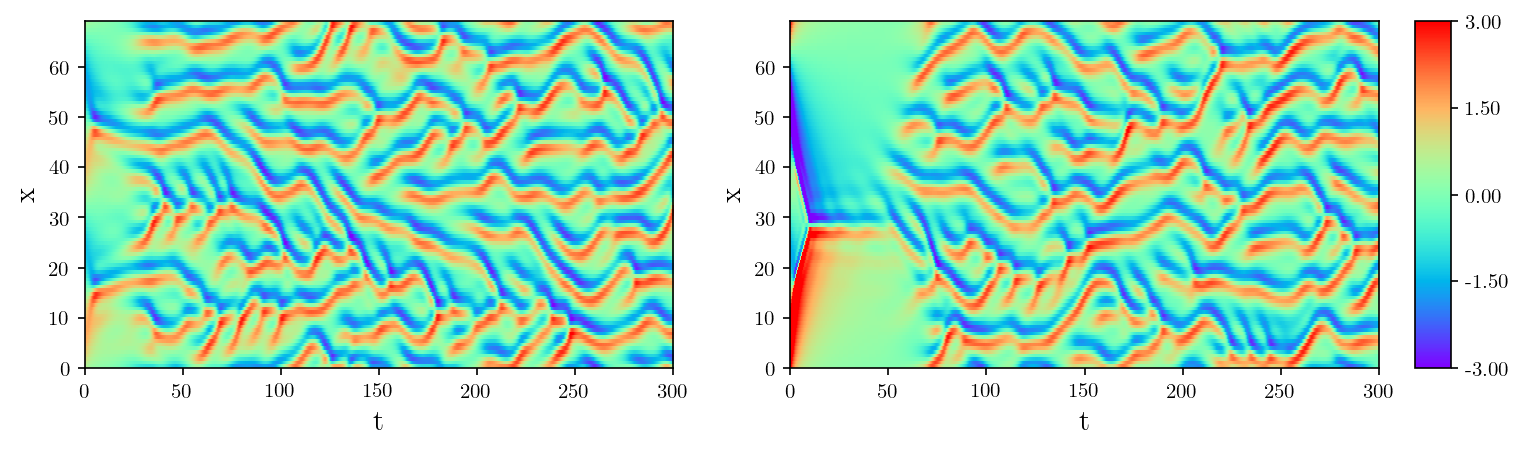
\includegraphics[width=0.8\textwidth]{Fig04.png}
    \caption{The Kuramoto-Sivashinsky equation for two different initial states solved using the spectral ETDRK4 scheme~\cite{cox2002exponential}.}
    \label{fig:ks-simulation}
\end{figure}
\end{frame}

\begin{frame}
\frametitle{Kuramoto-Sivashinsky Equation}

The AR-DenseED used for the K-S equation consists of a single convolutional block, followed by a dense block, followed by a deconvolutional block resulting in a model with just over $4800$ learnable weights.
The two previous states of the system are used as inputs, $\bm{\chi}^{n+1}=\left\{\bm{u}^{n},\bm{u}^{n-1}\right\}$.
Similar to the numerical solver, the time-step size of the model is set to $\Delta t = 0.1$ with a spatial discretization of $96$ points.
\end{frame}

\begin{frame}
\frametitle{Kuramoto-Sivashinsky Equation}
For the physics-constrained loss function, the implicit Crank-Nicolson time integration is used and the remaining spatial gradients are discretized as follows:
\begin{gather}
    \begin{gathered}
    T_{\Delta t}(\bm{\mathcal{U}}^{n}, F_{\Delta x}) = \bm{u}^{n} + \Delta t \left[-0.5\left(F_{\Delta x}(\bm{x}, \bm{u}^{n+1}) + F_{\Delta x}(\bm{x}, \bm{u}^{n})\right)\right],\\ F_{\Delta x}(\bm{x}, \bm{u}^{n}) = u^{n}u^{n}_{x} + u^{n}_{xx} + u^{n}_{xxxx},\end{gathered}\\
    uu_{x} = \frac{-u^{2}_{i+2}+8u^{2}_{i+1}-8u^{2}_{i-1}+u^{2}_{i-2}}{24 \Delta x}, \\
    u_{xx} = \frac{-u_{i+2}+16u_{i+1}-30u_{i}+16u_{i-1}-u_{i-2}}{12\Delta x^{2}},\\
    u_{xxxx} = \frac{-u_{i+3}+12u_{i+2}-39u_{i+1}+56u_{i}-39u_{i-1}+12u_{i-2}-u_{i-3}}{6\Delta x^{4}},
\end{gather}
\end{frame}

\begin{frame}
\frametitle{Kuramoto-Sivashinsky Equation}
where,
\begin{itemize}
\item{ the spatial gradients are approximated using fourth-order accurate finite difference discretizations that are implemented efficiently using convolutional operators.}

\item{The model was trained for $100$ epochs using $2560$ training scenarios that were generated using a truncated Fourier series with random coefficients discussed in~\ref{app:ks-initial}.}

\item{This Fourier series serves to approximate the physical turbulence of the system, and thus estimating the true distribution of the possible initial states $p(\bm{u}_{0})$.}

\item{During test time, we use $200$ test cases of true turbulent initial states of the system obtained from a numerical simulator.}

\end{itemize}
\end{frame}
\subsection{AR-DenseED Deterministic Predictions}

\begin{frame}
\frametitle{AR-DenseED Deterministic Predictions}
For each test case, we calculate the spatial mean square error (MSE) at each time-step defined as:
\begin{equation}
    \textrm{MSE}(t) = \frac{1}{N}\sum^{N}_{i=1}\left(u_{i}(t)-u^{*}_{i}(t)\right)^{2},
    \label{eq:mse}
\end{equation}
where $N$, $u$ and $u^*$ are the total number of points used to discretize the domain, target value from the numerical simulator and the AR-DenseED prediction, respectively.
\end{frame}

\begin{frame}
\frametitle{AR-DenseED Deterministic Predictions}
\begin{figure}[H]
    \centering
    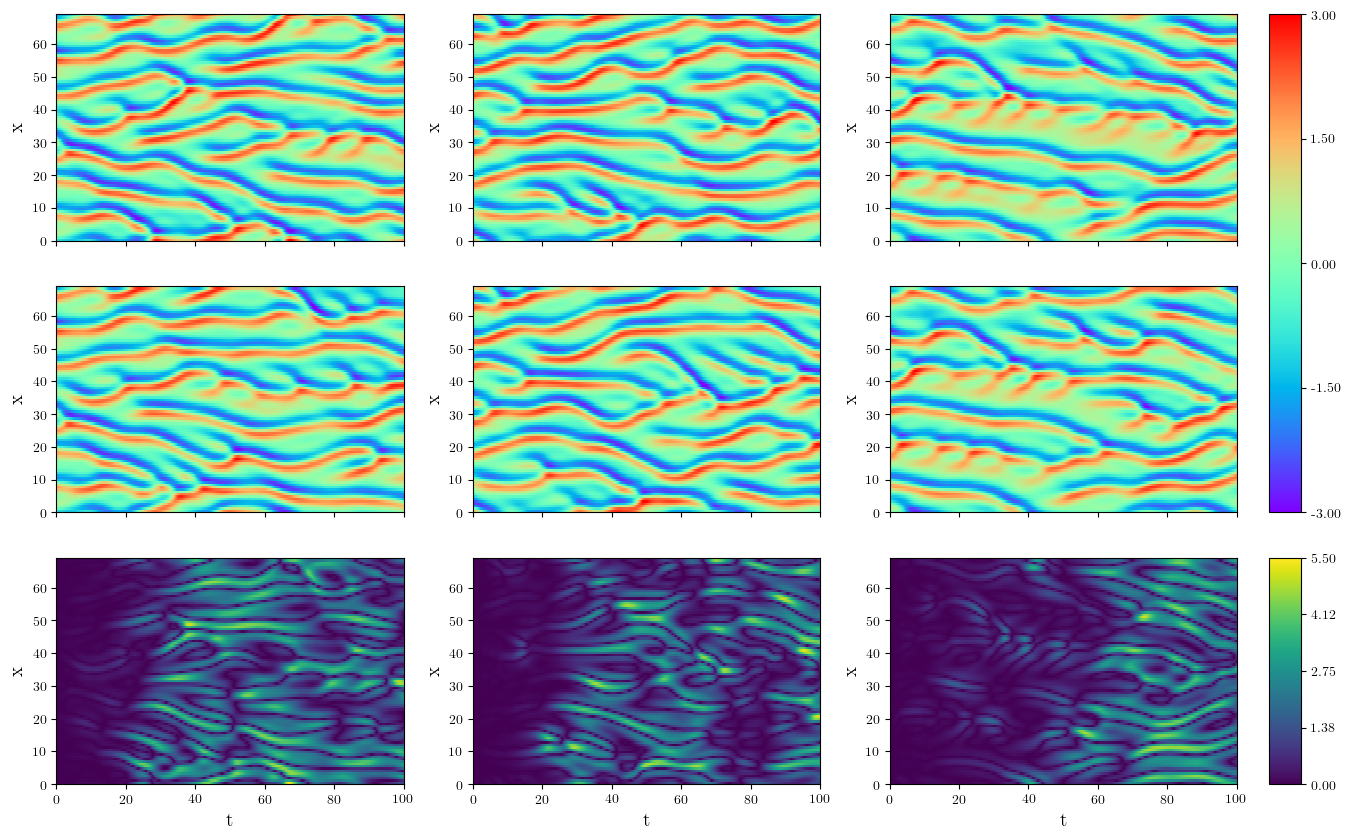
\includegraphics[width=0.8\textwidth]{Fig05.png}
    \caption{Three test predictions of the K-S equation using AR-DenseED. (Top to bottom) Target field solved system using the spectral ETDRK4 scheme, AR-DenseED prediction and finally the $L_1$ error.}
    \label{fig:ks-test-prediction}
\end{figure}
\end{frame}

\begin{frame}
\frametitle{AR-DenseED Deterministic Predictions}
\begin{figure}[H]
    \centering
    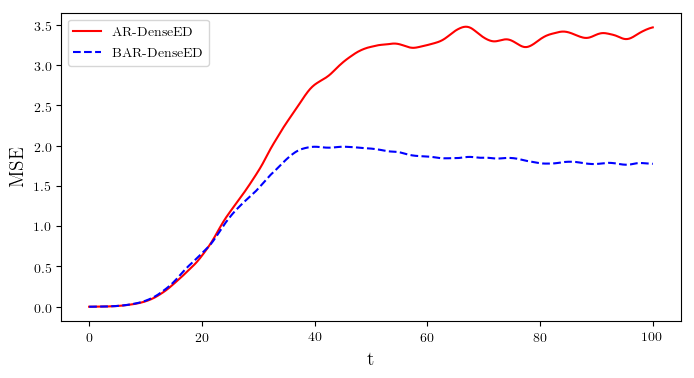
\includegraphics[width=0.7\textwidth]{Fig06.png}
    \caption{The mean MSE as a function of time for a test set of $200$ cases for the Kuramoto-Sivashinsky system.
    The error of BAR-DenseED is calculated using the expected value of the predictive distribution approximated using 30 samples of the posterior.}
    \label{fig:ks-mse}
\end{figure}
\end{frame}

\begin{frame}
\frametitle{AR-DenseED Deterministic Predictions}

\begin{table}[H]
    \caption{Wall-clock time for both spectral ETDRK4 scheme and AR-DenseED to simulate $5000$ time-steps of the Kuramoto-Sivashinsky system.
    Wall-clock time estimates were obtained by averaging $10$ independent simulation run times.}
    \resizebox{\columnwidth}{!}{
    \begin{tabular}{l|llcc}
               & \multicolumn{1}{c}{Hardware} & Backend & \multicolumn{1}{l}{$\Delta t$} & Wall-clock Time (s) \\ \hline
    Spectral   & Intel Xeon E5-2680           & Matlab  & $0.1$                           & \textbf{$0.185$}               \\
    AR-DenseED & Intel Xeon E5-2680           & PyTorch & $0.1$                           & $17.042$              \\
    AR-DenseED & GeForce GTX 1080 Ti          & PyTorch & $0.1$                           & $12.225$             
    \end{tabular}}
    \label{tab:ks-wallclock}
\end{table}

\end{frame}


\subsection{BAR-DenseED Probabilistic Predictions}

\begin{frame}
\frametitle{BAR-DenseED Probabilistic Predictions}

\begin{figure}[H]
    \centering
    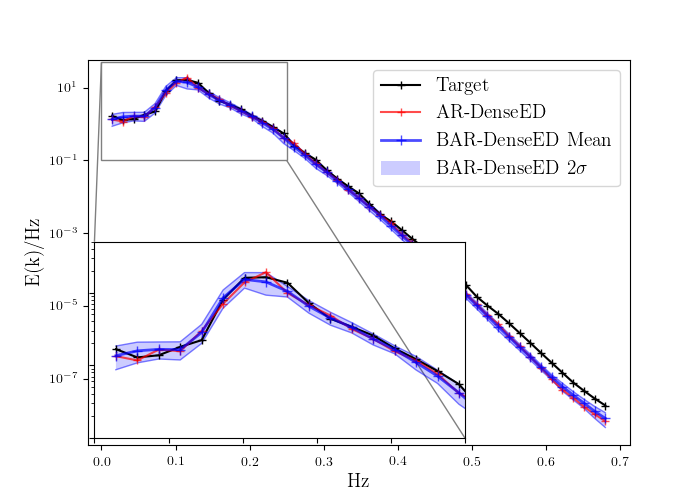
\includegraphics[width=0.7\textwidth]{Fig07.png}
    \caption{The time-averaged spectral energy density of the simulated result using the spectral ETDRK4 scheme (target), AR-DenseED deterministic prediction and BAR-DenseED empirical mean and standard deviation calculated from $30$ posterior samples.
    The averaged spectral energy density is the square of the modulus of the discrete Fourier transform over the domain, $x\in[0,22\pi]$, time-averaged between $t\in[0,500]$~\cite{brummitt2009search}.}
    \label{fig:ks-esd}
\end{figure}
\end{frame}


\begin{frame}
\frametitle{BAR-DenseED Probabilistic Predictions}
\begin{figure}[H]
    \centering
    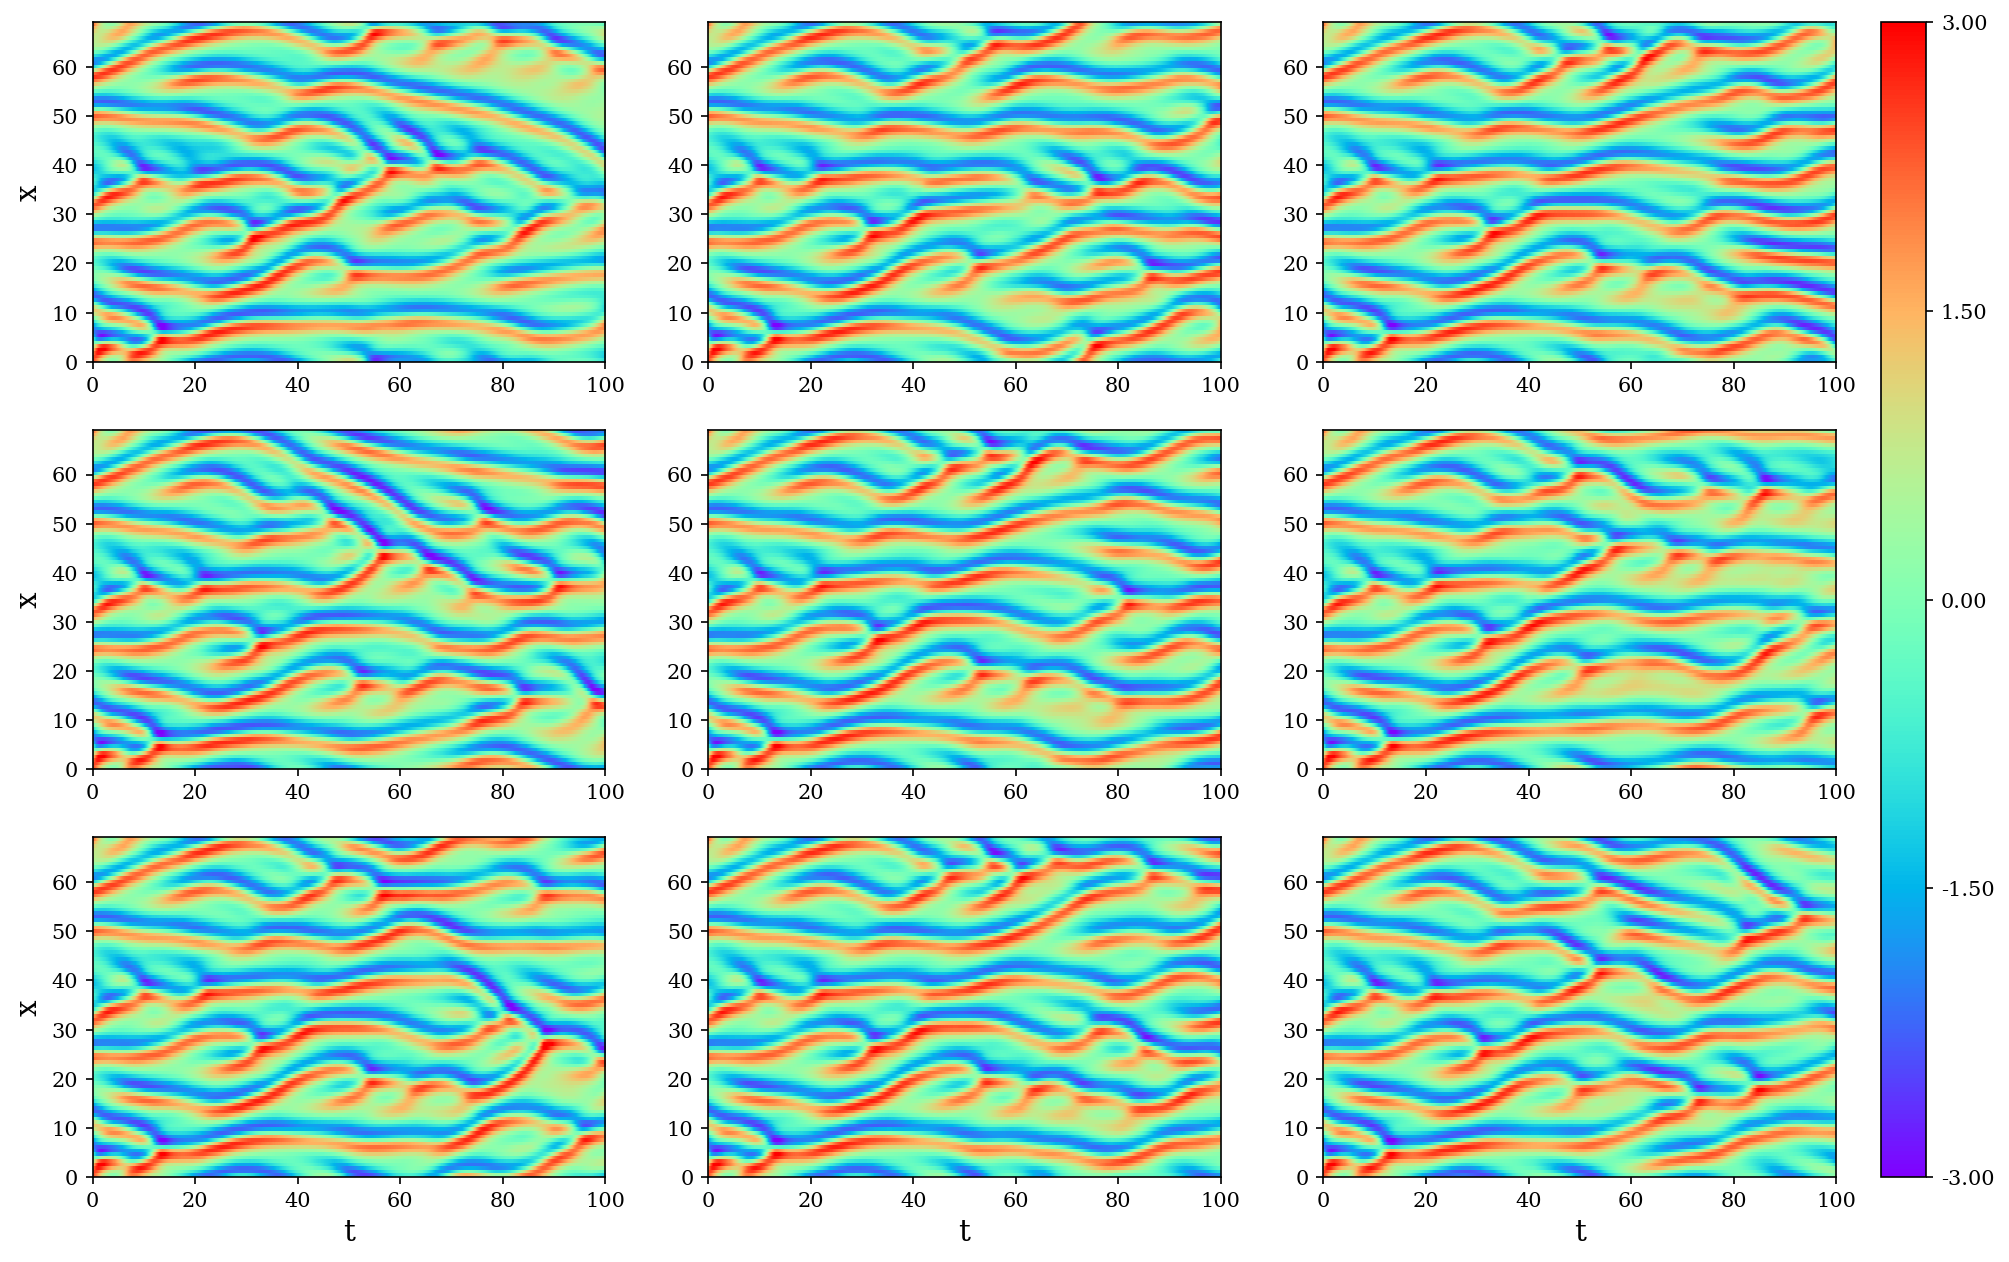
\includegraphics[width=0.7\textwidth]{Fig08.png}
    \caption{Samples from the posterior of BAR-DenseED approximated using SWAG for the Kuramoto-Sivashinsky system. The top left is the simulated result using the spectral ETDRK4 scheme.} 
    \label{fig:ks-bar-samples}
\end{figure}
\end{frame}


\section{1D Viscous Burgers' System}

\begin{frame}
\frametitle{1D Viscous Burgers' System}
Let us now consider the 1D viscous Burgers' equation in a periodic domain:
\begin{gather}
    \frac{\partial u}{\partial t} + u\frac{\partial u}{\partial x} - \viscosity \frac{\partial^{2} u}{\partial x^{2}} = 0,\\
     u(0,t) = u(L,t), \quad x\in[0,L], \quad t\in[0,T],
\end{gather}
where $u$ is the velocity and $\viscosity$ is the viscosity.
The Burgers' equation is a fundamental PDE that arises in multiple areas ranging from fluid dynamics to traffic flow. It is most recognized for its characteristic shock formations~\cite{whitham2011linear}.
\end{frame}

\begin{frame}
\frametitle{1D Viscous Burgers' System}
Consider a domain $x\in[0,1]$ with a constant viscosity of $\viscosity = 0.0025$ and the random initial condition given by a Fourier series with random coefficients:
\begin{equation}
    \begin{gathered}
    w(x) = a_0 + \sum_{l=1}^L a_l \sin(2l\pi x) + b_l \cos(2l\pi x), \\
    u(x,0) = \frac{2w(x)}{\max_x |w(x)|} + c,
    \label{eq:burger1d-initial}
    \end{gathered}
\end{equation}
where $a_l, b_l \sim \mc N(0, 1)$, $L=4$ and $c\sim \mc U(-1, 1)$.
\end{frame}

\begin{frame}
\frametitle{1D Viscous Burgers' System}
\begin{figure}[H]
    \centering
    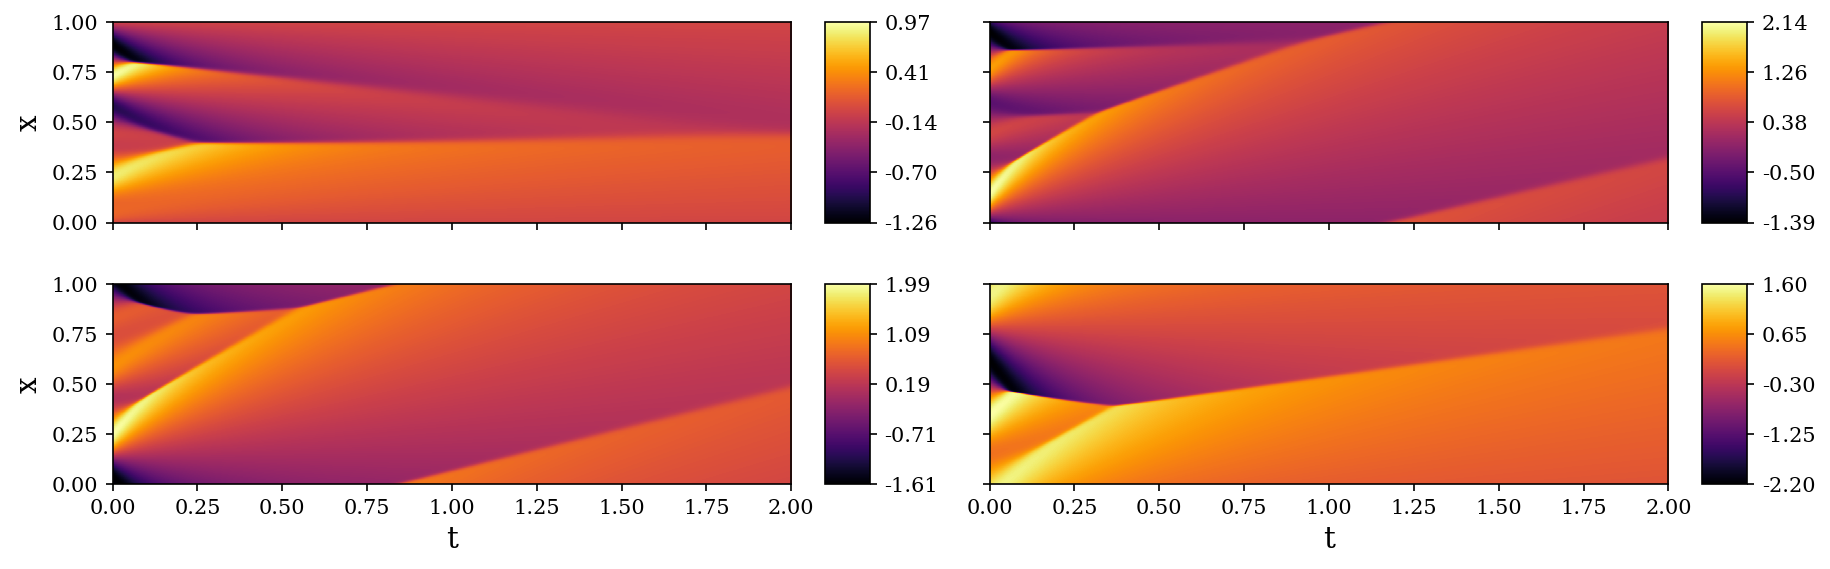
\includegraphics[width=\textwidth]{Fig09.png}
    \caption{1D viscous Burgers' equation simulations for four various initial conditions solved using Fenics finite element package~\cite{alnaes2015fenics}.}
    \label{fig:burgers1D-FEM}
\end{figure}
\end{frame}

\begin{frame}
\frametitle{1D Viscous Burgers' System}
Again the negative log of the joint posterior in~\Eqref{eq:posterior-form} is the loss function with the implicit Crank-Nicolson time integration.
The remaining spatial gradients are discretized as follows:
\begin{gather}
    \begin{gathered}T_{\Delta t}(\bm{\mathcal{U}}^{n}, F_{\Delta x}) = \bm{u}^{n} + \Delta t \left[-0.5\left(F_{\Delta x}(\bm{x}, \bm{u}^{n+1}) + F_{\Delta x}(\bm{x}, \bm{u}^{n})\right)\right],\\
    F_{\Delta x}(\bm{x}, \bm{u}^{n}) = u^{n}u^{n}_{x} - \viscosity u^{n}_{xx},\end{gathered}\\
    uu_{x} = \frac{u^{2}_{i+1} - u^{2}_{i-1}}{4\Delta x}, \quad u_{xx} = \frac{u_{i+1} - 2u_{i} + u_{i-1}}{\Delta x^{2}},
\end{gather}
where the spatial gradients are approximated using second-order accurate approximations that are implemented efficiently using convolutional operators.
\end{frame}

\subsection{AR-DenseED Deterministic Predictions}

\begin{frame}
\frametitle{AR-DenseED Deterministic Predictions}
\begin{figure}[H]
    \centering
    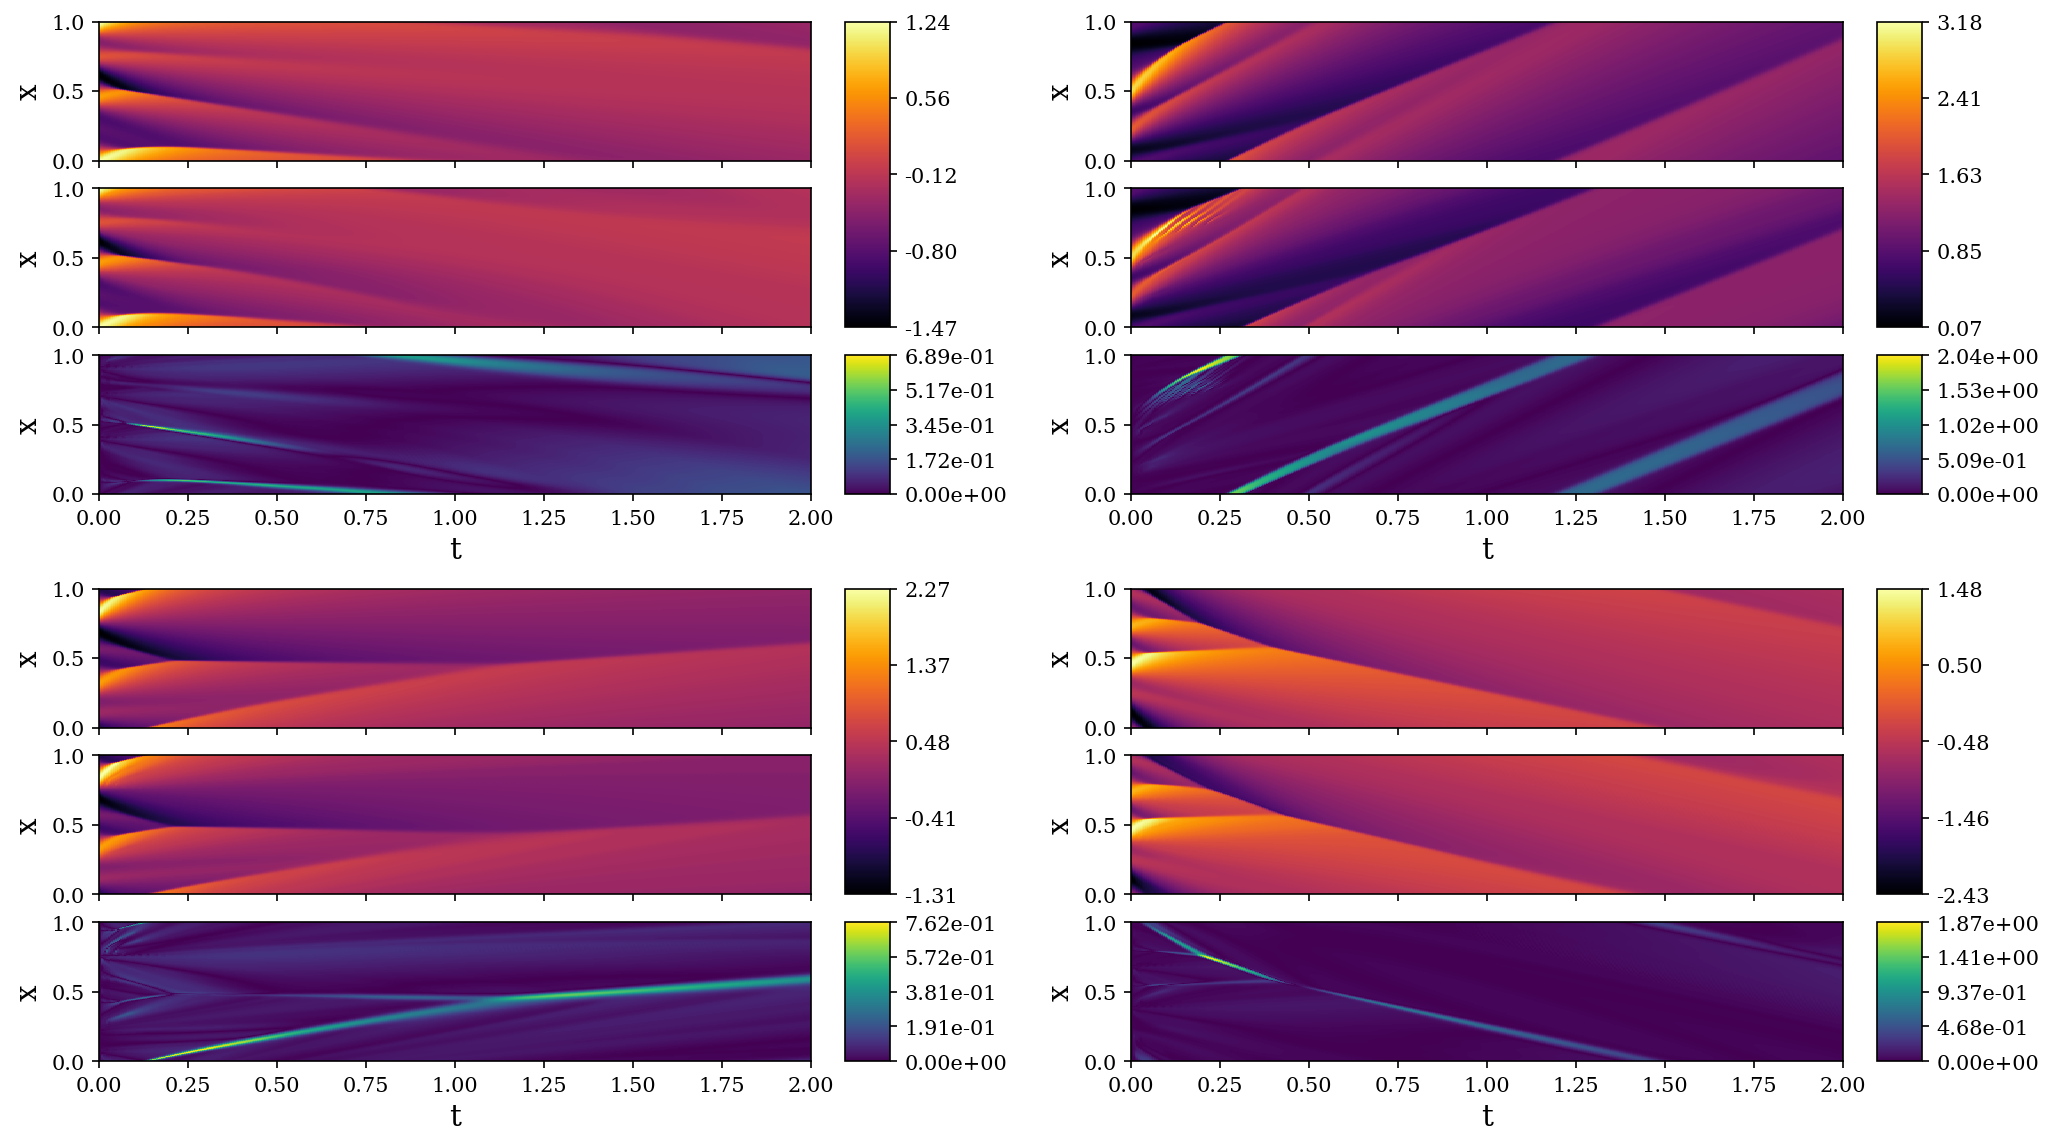
\includegraphics[width=0.8\textwidth]{Fig10.png}
    \caption{AR-DenseED predictions for four test initial conditions of the 1D Burgers' system. (Top to bottom) FEM target solution, AR-DenseED prediction, and $L_1$ error.}
    \label{fig:burgers1D-ARDenseED}
\end{figure}
\end{frame}

\begin{frame}
\frametitle{AR-DenseED Deterministic Predictions}
The MSE can be slightly misleading to the actual quality of the prediction for this system since a small deviation in shock trajectory can potentially yield a growing error.
Thus, we also compute the energy square error (ESE) for a 1D domain:
\begin{align}
    \begin{split}
        \textrm{ESE}(t) &= \left[\int_{0}^{1} \frac{(u(x,t))^{2}}{2} dx - \int_{0}^{1}\frac{(u^{*}(x,t))^{2}}{2} dx\right]^{2},\\
        &= \left[\frac{1}{N}\sum^{N}_{i=1}\frac{(u_{i}(t))^{2}}{2} - \frac{1}{N}\sum^{N}_{i=1}\frac{(u_{i}^{*}(t))^{2}}{2}\right]^{2},
        \label{eq:ese}
    \end{split}
\end{align}
which instead captures the discrepancy of the total energy, $u^{2}/2$, within the domain, making this metric invariant to shock location.

\end{frame}

\begin{frame}
\frametitle{AR-DenseED Deterministic Predictions}
%
\begin{figure}[H]
    \centering
    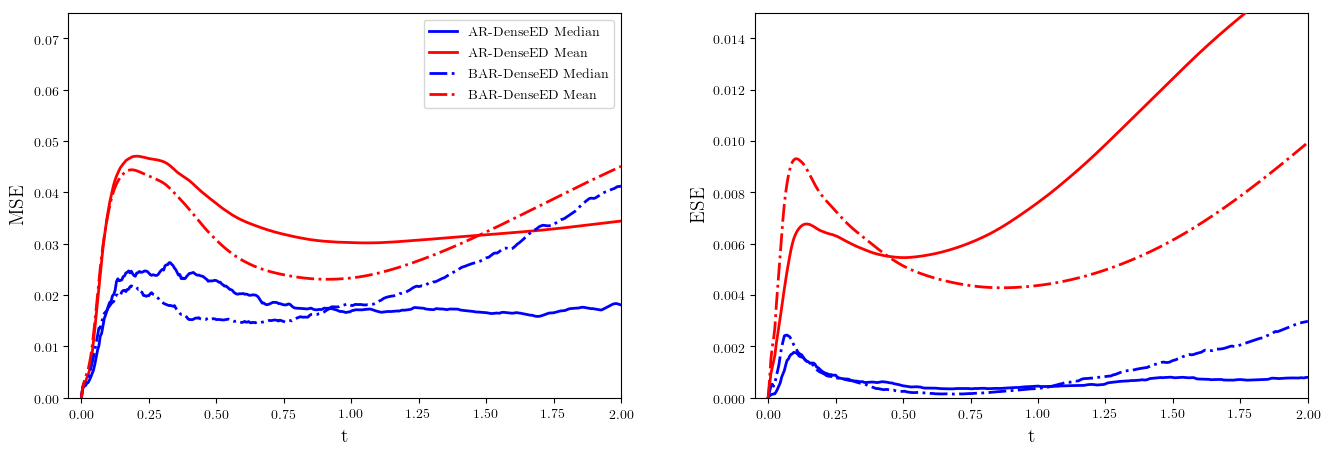
\includegraphics[width=0.9\textwidth]{Fig11.png}
    \caption{(Left to right) The mean square error (MSE) and energy squared error (ESE) as a function of time for a test set of $200$ cases for the 1D Burgers' system.
    The error of BAR-DenseED is calculated using the expected value of the predictive distribution approximating using $30$ samples of the posterior.}
    \label{fig:burgers1D-MSE}
\end{figure}
\end{frame}

\begin{frame}
\frametitle{AR-DenseED Deterministic Predictions}
\begin{table}[H]
    \caption{Wall-clock time of finite element, finite difference and AR-DenseED to simulate $400$ time-steps of the 1D-Burgers' system.
    Wall-clock time estimates were obtained by averaging $10$ independent simulation run times.}
    \resizebox{\columnwidth}{!}{
    \begin{tabular}{l|llcc}
                     & \multicolumn{1}{c}{Hardware} & Backend & \multicolumn{1}{c}{$\Delta t$} & Wall-clock (s) \\ \hline
    Finite Element    & Intel Xeon E5-2680  & Fenics  & $0.0005$  & $43.696$ \\
    Finite Element    & Intel Xeon E5-2680  & Fenics  & $0.001$  & $22.645$ \\
    Finite Element    & Intel Xeon E5-2680  & Fenics  & $0.005$   & $7.450$ \\
    Finite Difference & Intel Xeon E5-2680  & PyTorch & $0.0005$ & $4.856$ \\
    Finite Difference & GeForce GTX 1080 Ti  & PyTorch & $0.0005$ & $12.8359$ \\
    Finite Difference & Intel Xeon E5-2680  & PyTorch & $0.001$  & $2.862$ \\
    Finite Difference & GeForce GTX 1080 Ti   & PyTorch & $0.001$  & $6.264$\\
    AR-DenseED        & Intel Xeon E5-2680  & PyTorch & $0.005$  & $1.286$  \\
    AR-DenseED        & GeForce GTX 1080 Ti   & PyTorch & $0.005$  & $0.705$
    \end{tabular}}
    \label{tab:burger1d-wallclock}
\end{table}
\end{frame}

\subsection{BAR-DenseED Probabilistic Predictions}

\begin{frame}
\frametitle{BAR-DenseED Probabilistic Predictions}
%
\begin{figure}[H]
    \centering
    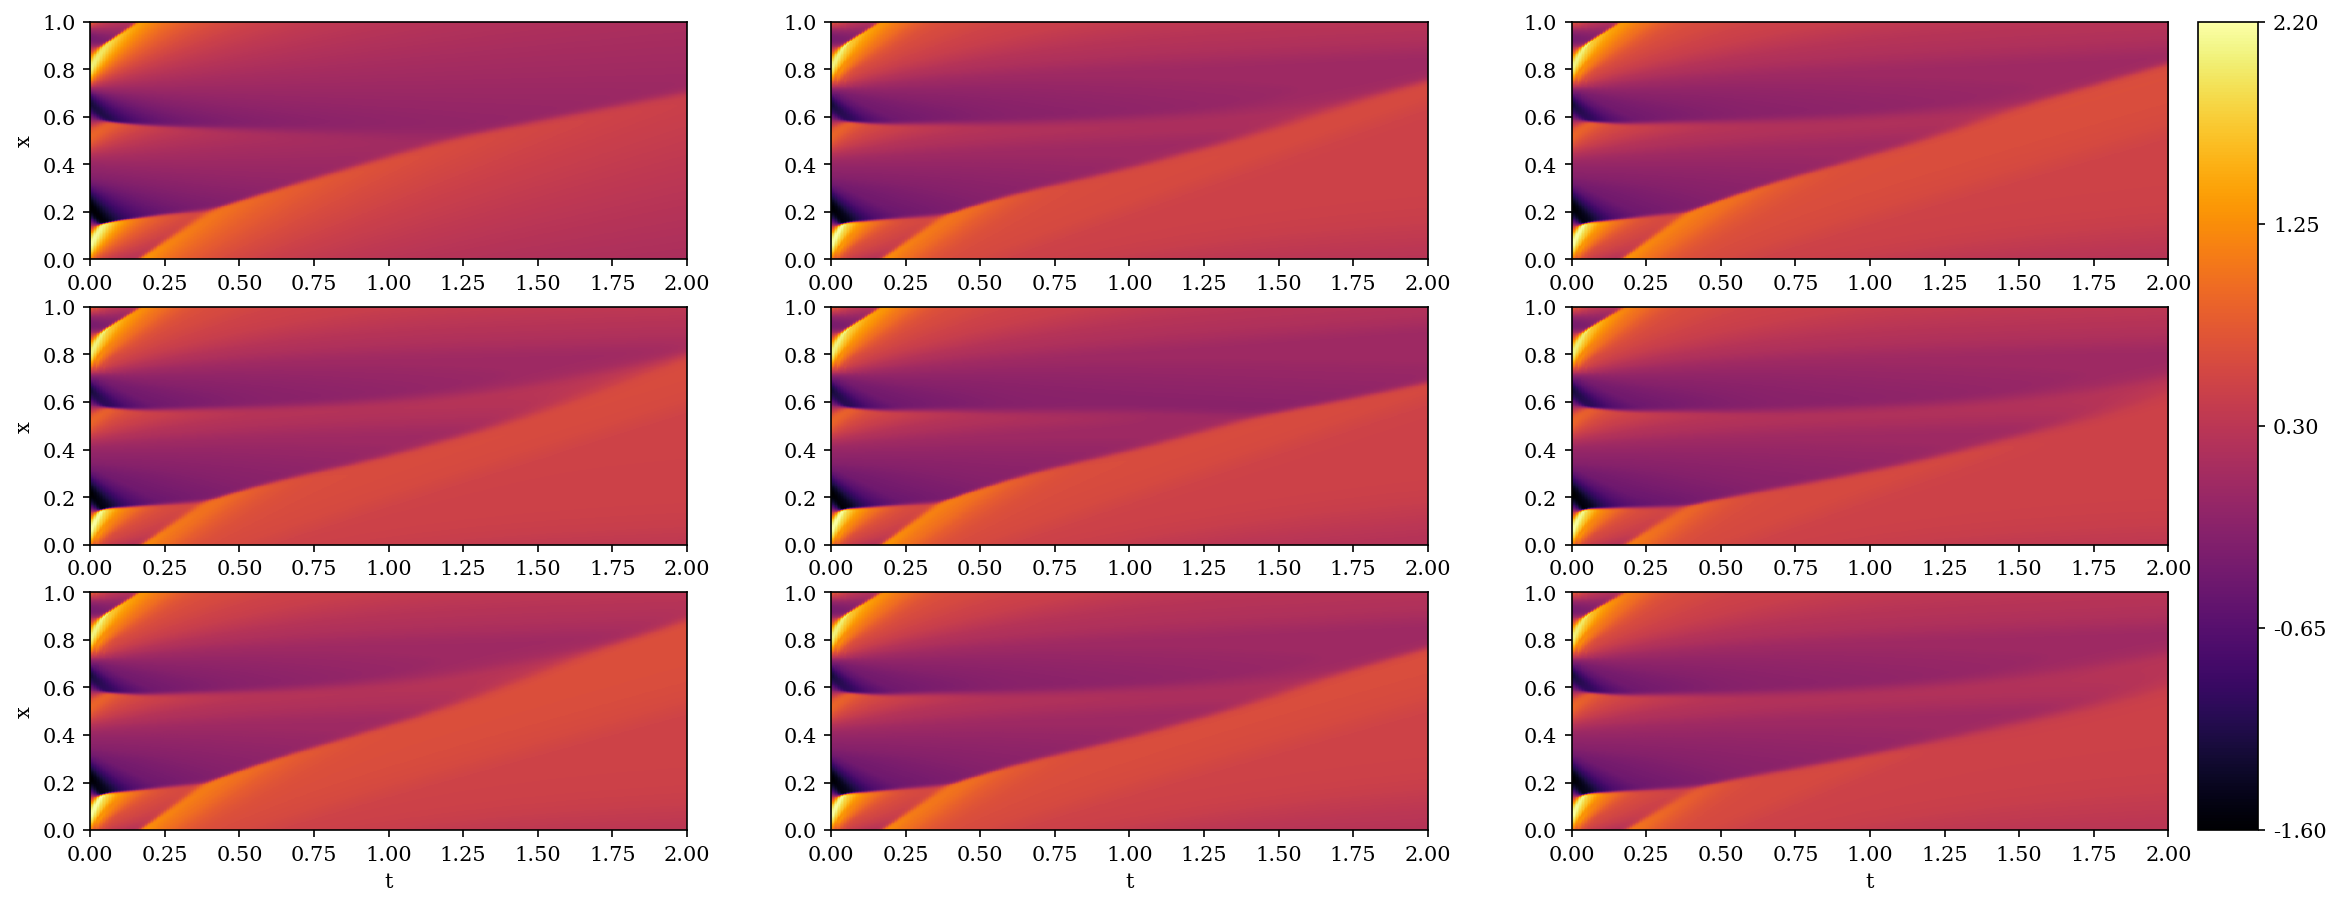
\includegraphics[width=0.9\textwidth]{Fig12.png}
    \caption{Samples from the posterior of BAR-DenseED approximated using SWAG for the 1D Burgers' system. The top left is the simulated result using the finite element method.} 
    \label{fig:burgers1D-bar-samples}
\end{figure}
\end{frame}

\begin{frame}
\frametitle{BAR-DenseED Probabilistic Predictions}
\begin{figure}[H]
    \centering
    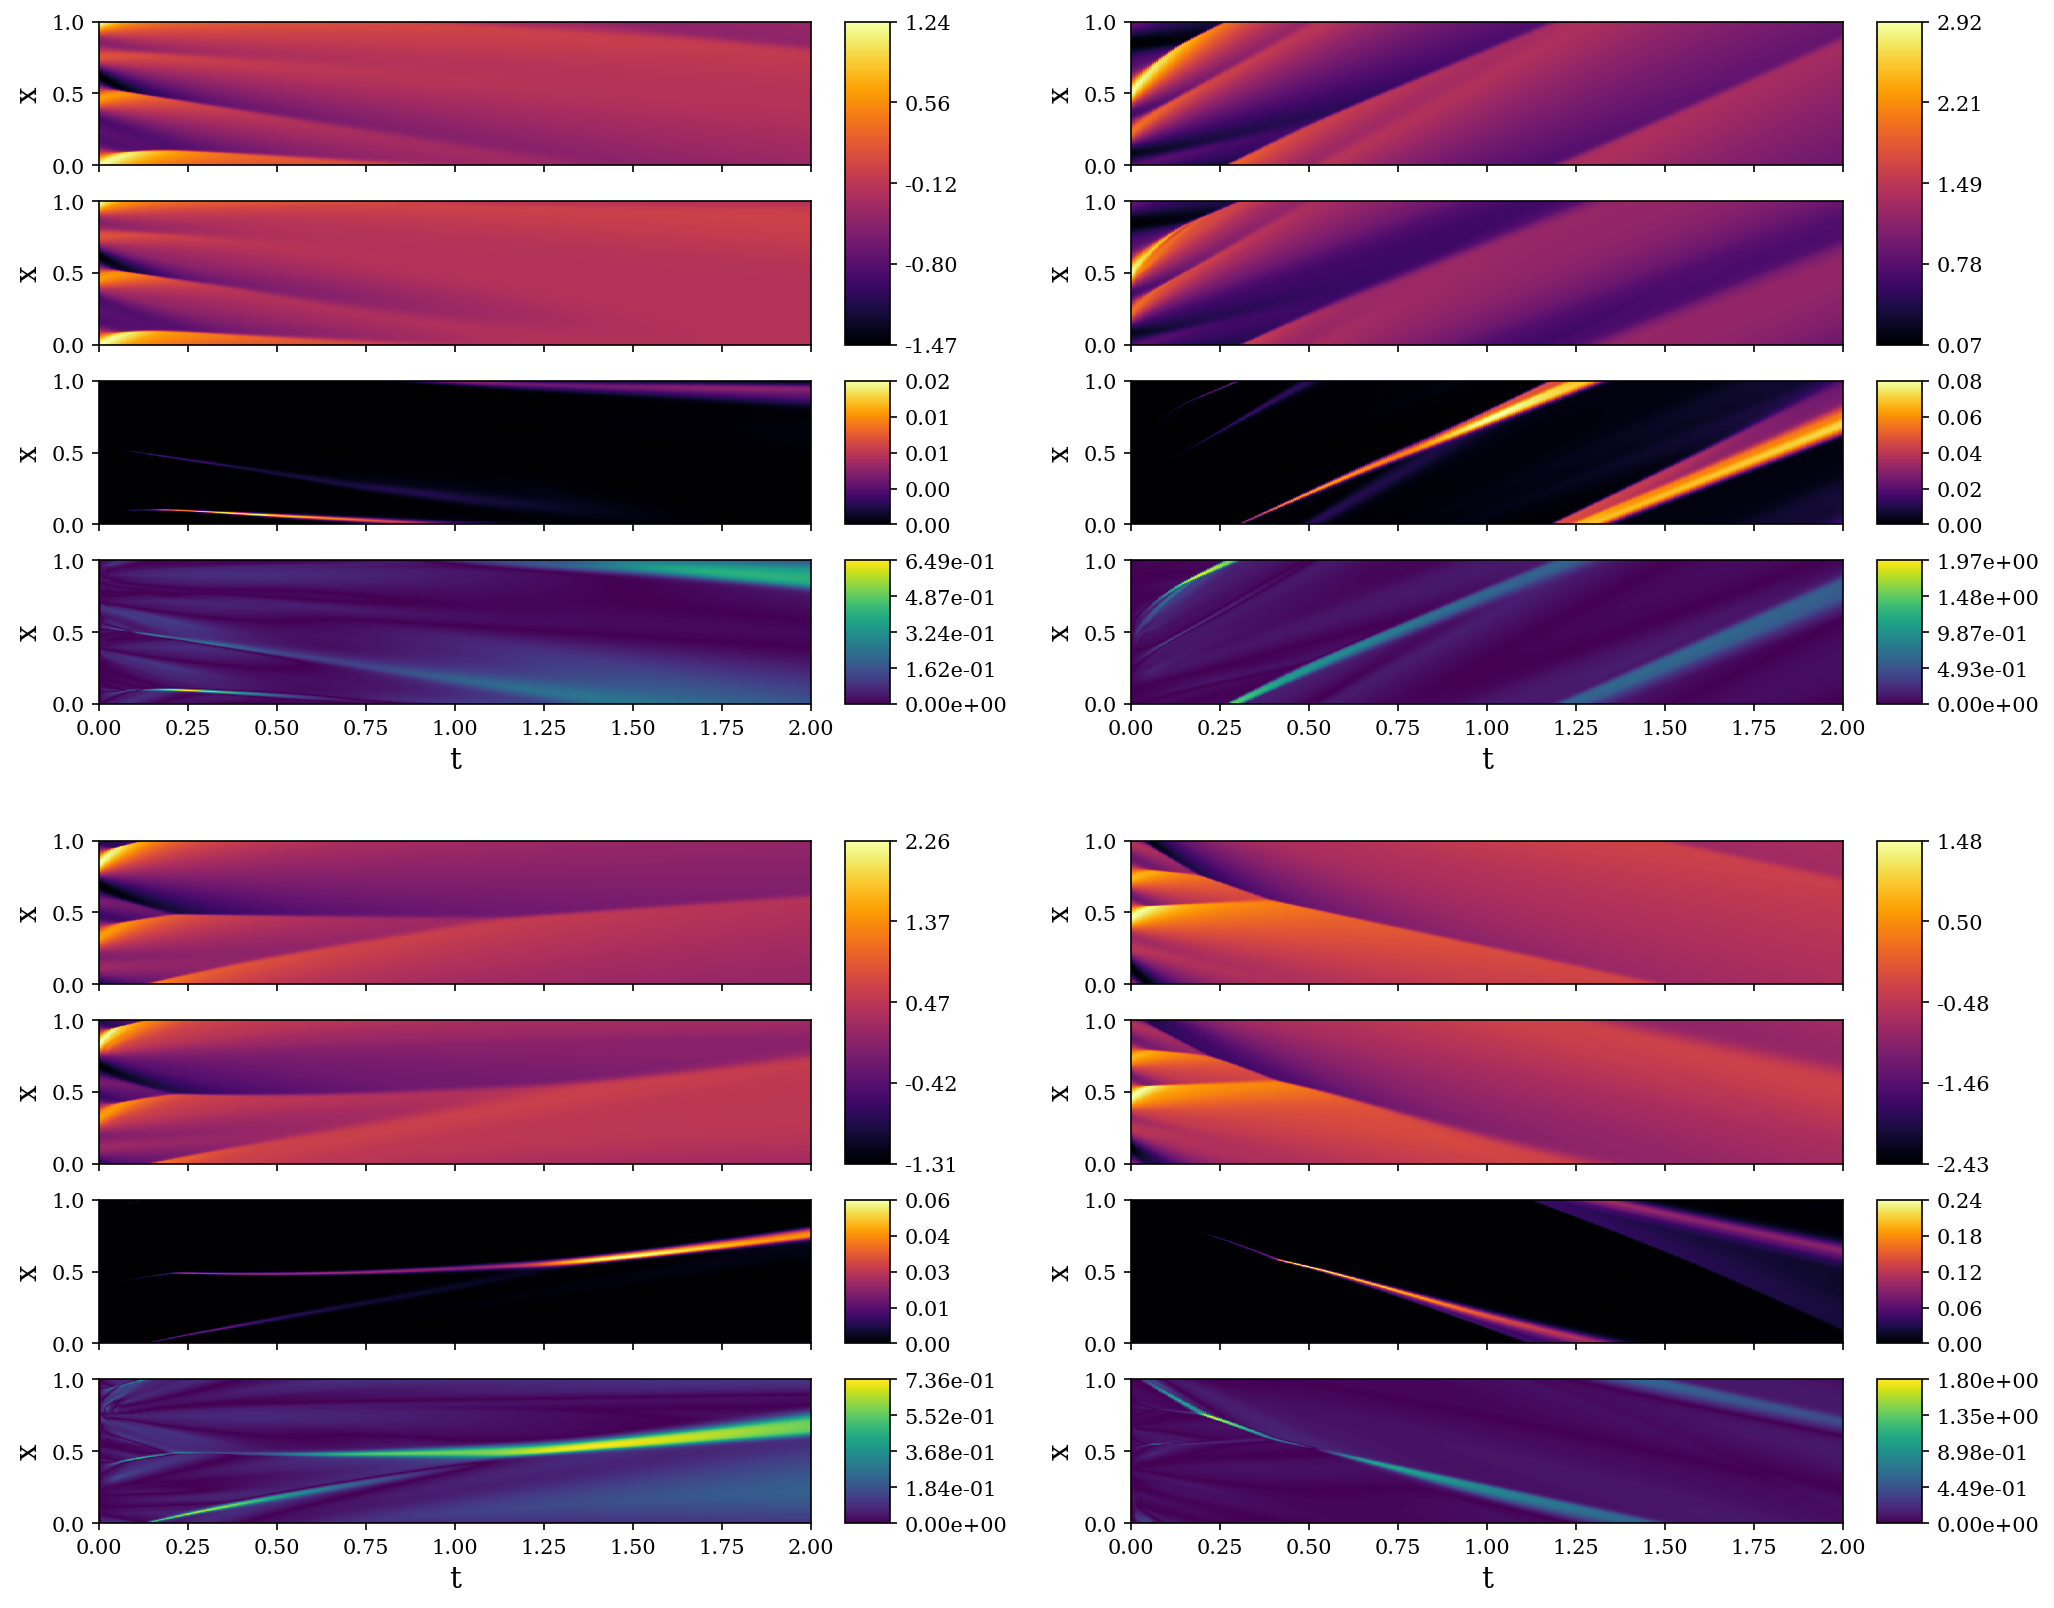
\includegraphics[width=0.7\textwidth]{Fig13.png}
    \caption{BAR-DenseED predictions for four test initial conditions of the 1D Burgers' system. (Top to bottom) FEM target solution, BAR-DenseED expected response, BAR-DenseED variance and $L_1$ error between the target and expected values.}
    \label{fig:burgers1D-BARDenseED}
\end{figure}
\end{frame}


\begin{frame}
\frametitle{BAR-DenseED Probabilistic Predictions}

\begin{figure}[H]
    \centering
    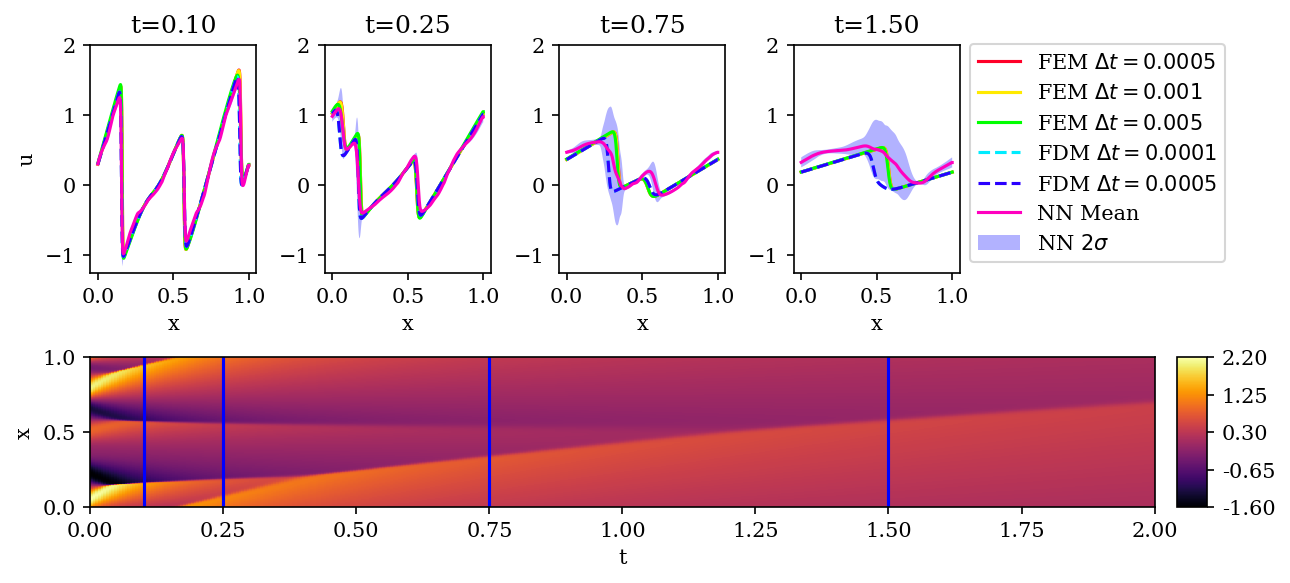
\includegraphics[width=\textwidth]{Fig14.png}
    \caption{Instantaneous profiles of both the finite element method (FEM) and finite difference method (FDM) numerical solvers along with BAR-DenseED neural network (NN) predictive expectation and standard deviation at four various times of a test case.
    The bottom contour is the ideal target calculated using FEM with a time-step size $\Delta t =0.0005$.
    The blue lines mark each profile location.}
    \label{fig:burgers1D-profile1}
\end{figure}
\end{frame}


\begin{frame}
\frametitle{BAR-DenseED Probabilistic Predictions}
\begin{figure}[H]
    \centering
    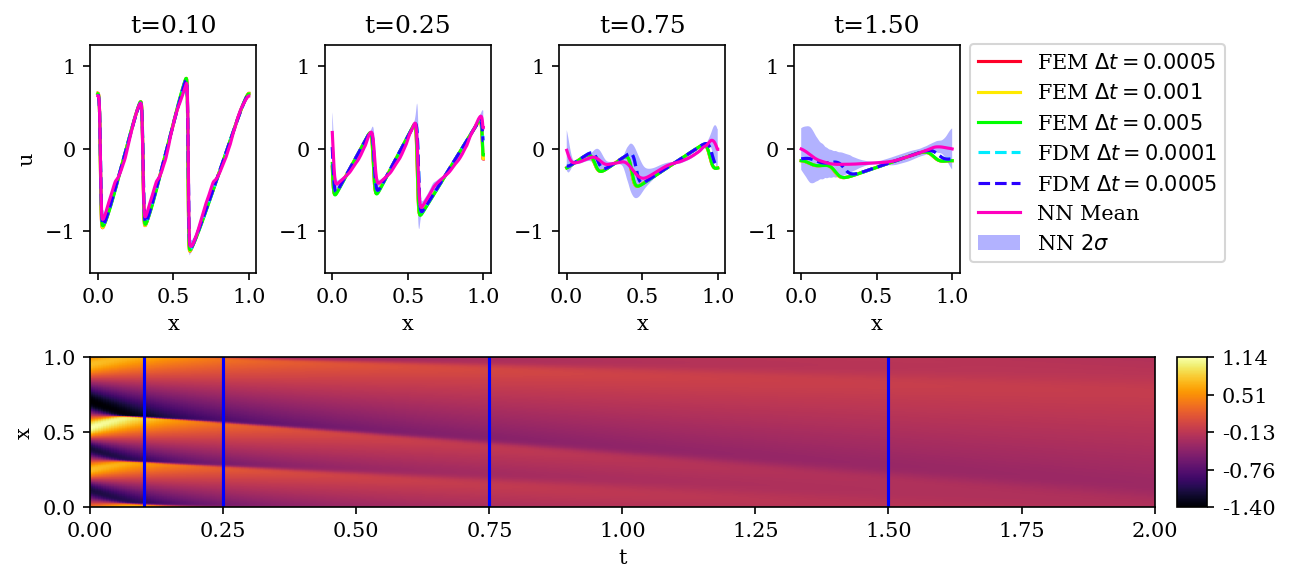
\includegraphics[width=\textwidth]{Fig15.png}
    \caption{Instantaneous profiles of both finite element method (FEM) and finite difference method (FDM) numerical solvers along with BAR-DenseED neural network (NN) predictive expectation and standard deviation at four various times of a test case.
    The bottom contour is the ideal target calculated using FEM with a time-step size $\Delta t =0.0005$.
    The blue lines mark each profile location.}
    \label{fig:burgers1D-profile2}
\end{figure}
\end{frame}


\section{2D Coupled Burgers' System}

\begin{frame}
\frametitle{2D Coupled Burgers' System}
Lastly, we will consider the 2D coupled Burgers' system:
\begin{gather}
    \bm{u}_t + \bm{u}\cdot \nabla \bm{u} - \viscosity \Delta \bm{u} = 0,\\
    \bm{u}(0,y,t) = \bm{u}(L,y,t), \quad \bm{u}(x,0,t) = \bm{u}(x,L,t), \\
    \left\{x,y \right\} \in [0,L], \quad t\in[0,T],
\end{gather}
which when expanded into its components takes the following form:
\begin{equation}
    \begin{aligned}
        {\frac{\partial u}{\partial t}+u \frac{\partial u}{\partial x}+v \frac{\partial u}{\partial y} - \viscosity \left(\frac{\partial^{2} u}{\partial x^{2}}+\frac{\partial^{2} u}{\partial y^{2}}\right)} = 0, \\ 
        {\frac{\partial v}{\partial t}+u \frac{\partial v}{\partial x}+v \frac{\partial v}{\partial y} - \viscosity \left(\frac{\partial^{2} v}{\partial x^{2}}+\frac{\partial^{2} v}{\partial y^{2}}\right)} = 0,
    \end{aligned}
\end{equation}

\end{frame}

\begin{frame}
\frametitle{2D Coupled Burgers' System}
where,
 $\viscosity$ is the viscosity of the system which will be held at $\nu=0.005$ and the domain size set to $\left\{x,y \right\} \in [0,1]$.
$u$ and $v$ are the $x$ and $y$ velocity components, respectively.

The 2D coupled Burgers' equation is an excellent benchmark PDE due to both
\begin{itemize}
\item{its non-linear term as well as}
\item{diffusion operator,}
\end{itemize} 
making it much more complex than the standard advection or diffusion equations.

\end{frame}


\begin{frame}
\frametitle{2D Coupled Burgers' System}
As in our previous examples, we are interested in surrogate modeling for various initial conditions.
We will initialize the field using a truncated Fourier series with random coefficients:
\begin{equation}
    \begin{gathered}
        \bm{w}(x,y) = \sum_{i=-L}^L \sum_{j=-L}^L \bm{a}_{ij} \sin(2\pi\left(ix + jy\right)) + \bm{b}_{ij} \cos(2\pi\left(ix + jy\right)), \\
        \bm{u}(x, y, 0) = \frac{2\bm{w}(x,y)}{\max_{\left\{x,y\right\}} |\bm{w}(x,y)|} + \bm{c},
    \end{gathered}
    \label{eq:burger2d-initial}
\end{equation}
where $\bm{a}_{ij}, \bm{b}_{ij} \sim \mc N(0, \bm{I}_{2})$, $L=4$ and $\bm{c}\sim \mc U(-1, 1) \in \mathbb{R}^{2}$.
Several of these randomly generated initial conditions are illustrated in Fig.~\ref{fig:burgers2D-Initial}.
\end{frame}


\begin{frame}
\frametitle{2D Coupled Burgers' System}
\begin{figure}[H]
    \centering
    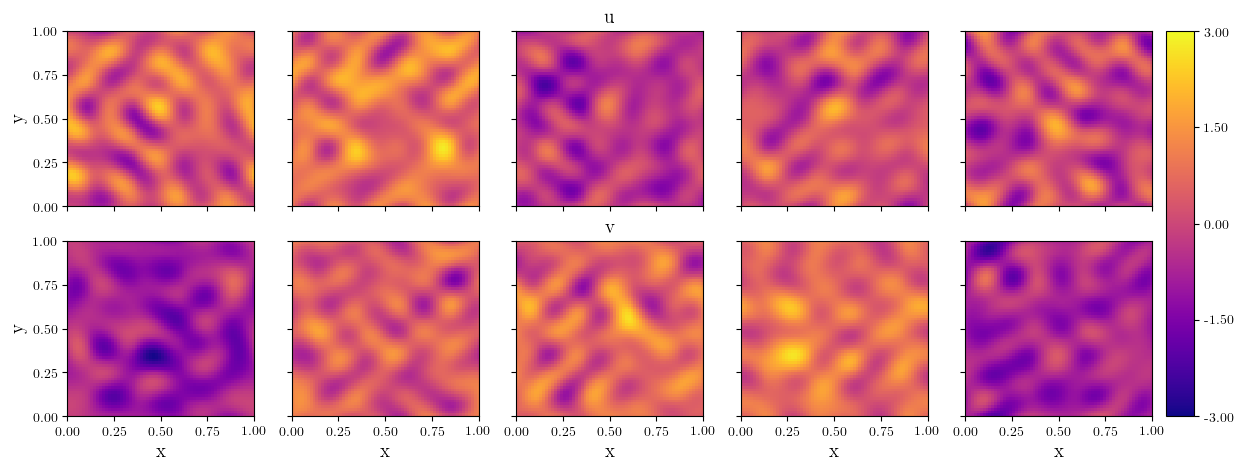
\includegraphics[width=0.9\textwidth]{Fig16.png}
    \caption{Randomly generated initial conditions for the 2D coupled Burgers' system. (Top to bottom) The $x$-velocity and $y$-velocity components. (Left to right) Different samples of the random initial condition.}
    \label{fig:burgers2D-Initial}
\end{figure}
\end{frame}


\begin{frame}
\frametitle{2D Coupled Burgers' System}
\begin{figure}[H]
    \centering
    \begin{subfigure}{0.7\textwidth}
        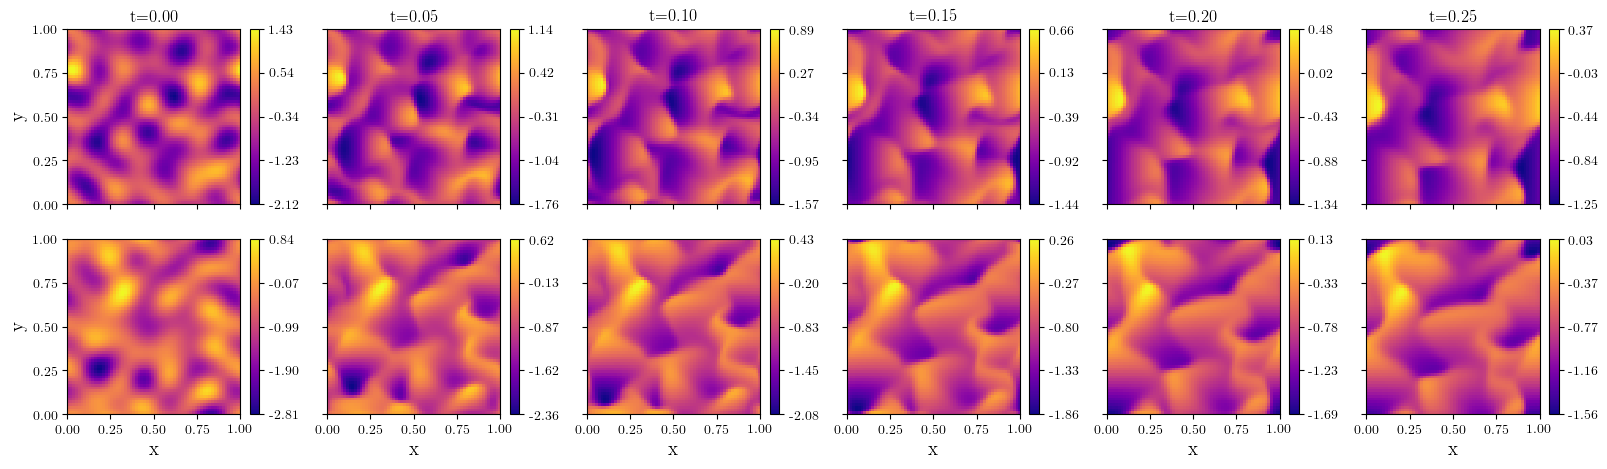
\includegraphics[width=\textwidth]{Fig17a.png}
        \vspace*{-7mm}
        \subcaption{Simulation 1}
    \end{subfigure}
    \begin{subfigure}{0.7\textwidth}
        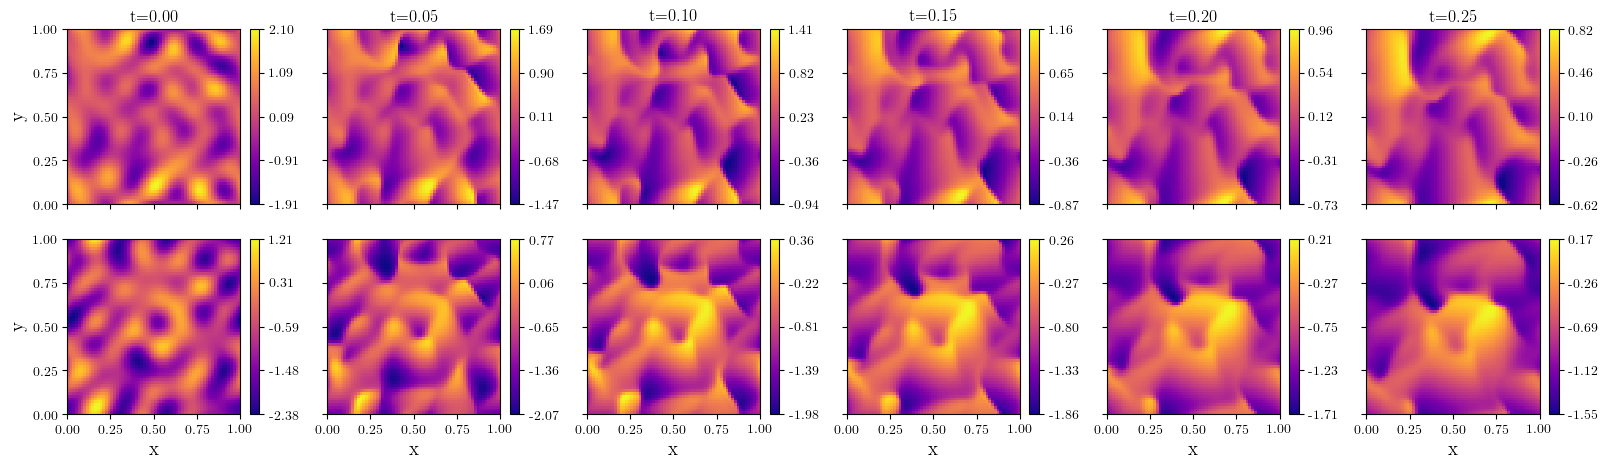
\includegraphics[width=\textwidth]{Fig17b.png}
        \vspace*{-7mm}
        \subcaption{Simulation 2}
    \end{subfigure}
    \caption{2D coupled Burgers' equation simulations for two various initial conditions solved using the Fenics finite element package~\cite{alnaes2015fenics}.
    (Top to bottom) $x$-velocity and $y$-velocity components.}
    \label{fig:burgers2D-fenics}
\end{figure}
\end{frame}


\begin{frame}
\frametitle{2D Coupled Burgers' System}
\begin{gather}
    \begin{gathered}
    T_{\Delta t}(\bm{\mathcal{U}}^{n}, F_{\Delta x}) = \bm{u}^{n} + \Delta t \left[-0.5\left(F_{\Delta x}(\bm{x}, \bm{u}^{n+1}) + F_{\Delta x}(\bm{x}, \bm{u}^{n})\right)\right],\\
    F_{\Delta x}(\bm{x}, \bm{u}^{n}) = \bm{u}^{n}\cdot \nabla \bm{u}^{n} - \viscosity \Delta \bm{u}^{n},
    \end{gathered}\\
    \bm{u}_{x}=\frac{1}{8\Delta x}\begin{bmatrix} 
    -1 & 0 & 1 \\
    -2 & 0 & 2 \\
    -1 & 0 & 1
    \end{bmatrix}\ast \bm{u}, \quad 
    \bm{u}_{y}=\frac{1}{8\Delta x}\begin{bmatrix} 
        -1 & -2 & -1 \\
        0 & 0 & 0 \\
        1 & 2 & 1
    \end{bmatrix}\ast \bm{u}, \\
    \Delta \bm{u}=\frac{1}{2\Delta x^{2}}\begin{bmatrix} 
        1 & 0 & 1 \\
        0 & -4 & 0 \\
        1 & 0 & 1
    \end{bmatrix}\ast \bm{u},
\end{gather}
\end{frame}


\begin{frame}
\frametitle{2D Coupled Burgers' System}

where,
 the spatial gradients are approximated using Sobel filter 2D convolutions which are analogous to smoothed second-order accurate finite difference approximations~\cite{sobel19683x3}.

\textbf{Using the Sobel filter was found to increase the stability of training and significantly reduce spurious oscillations in the model's predictions.}
\end{frame}

\subsection{AR-DenseED Deterministic Predictions}
\begin{frame}
\frametitle{AR-DenseED Deterministic Predictions}
%
\begin{figure}[H]
    \centering
    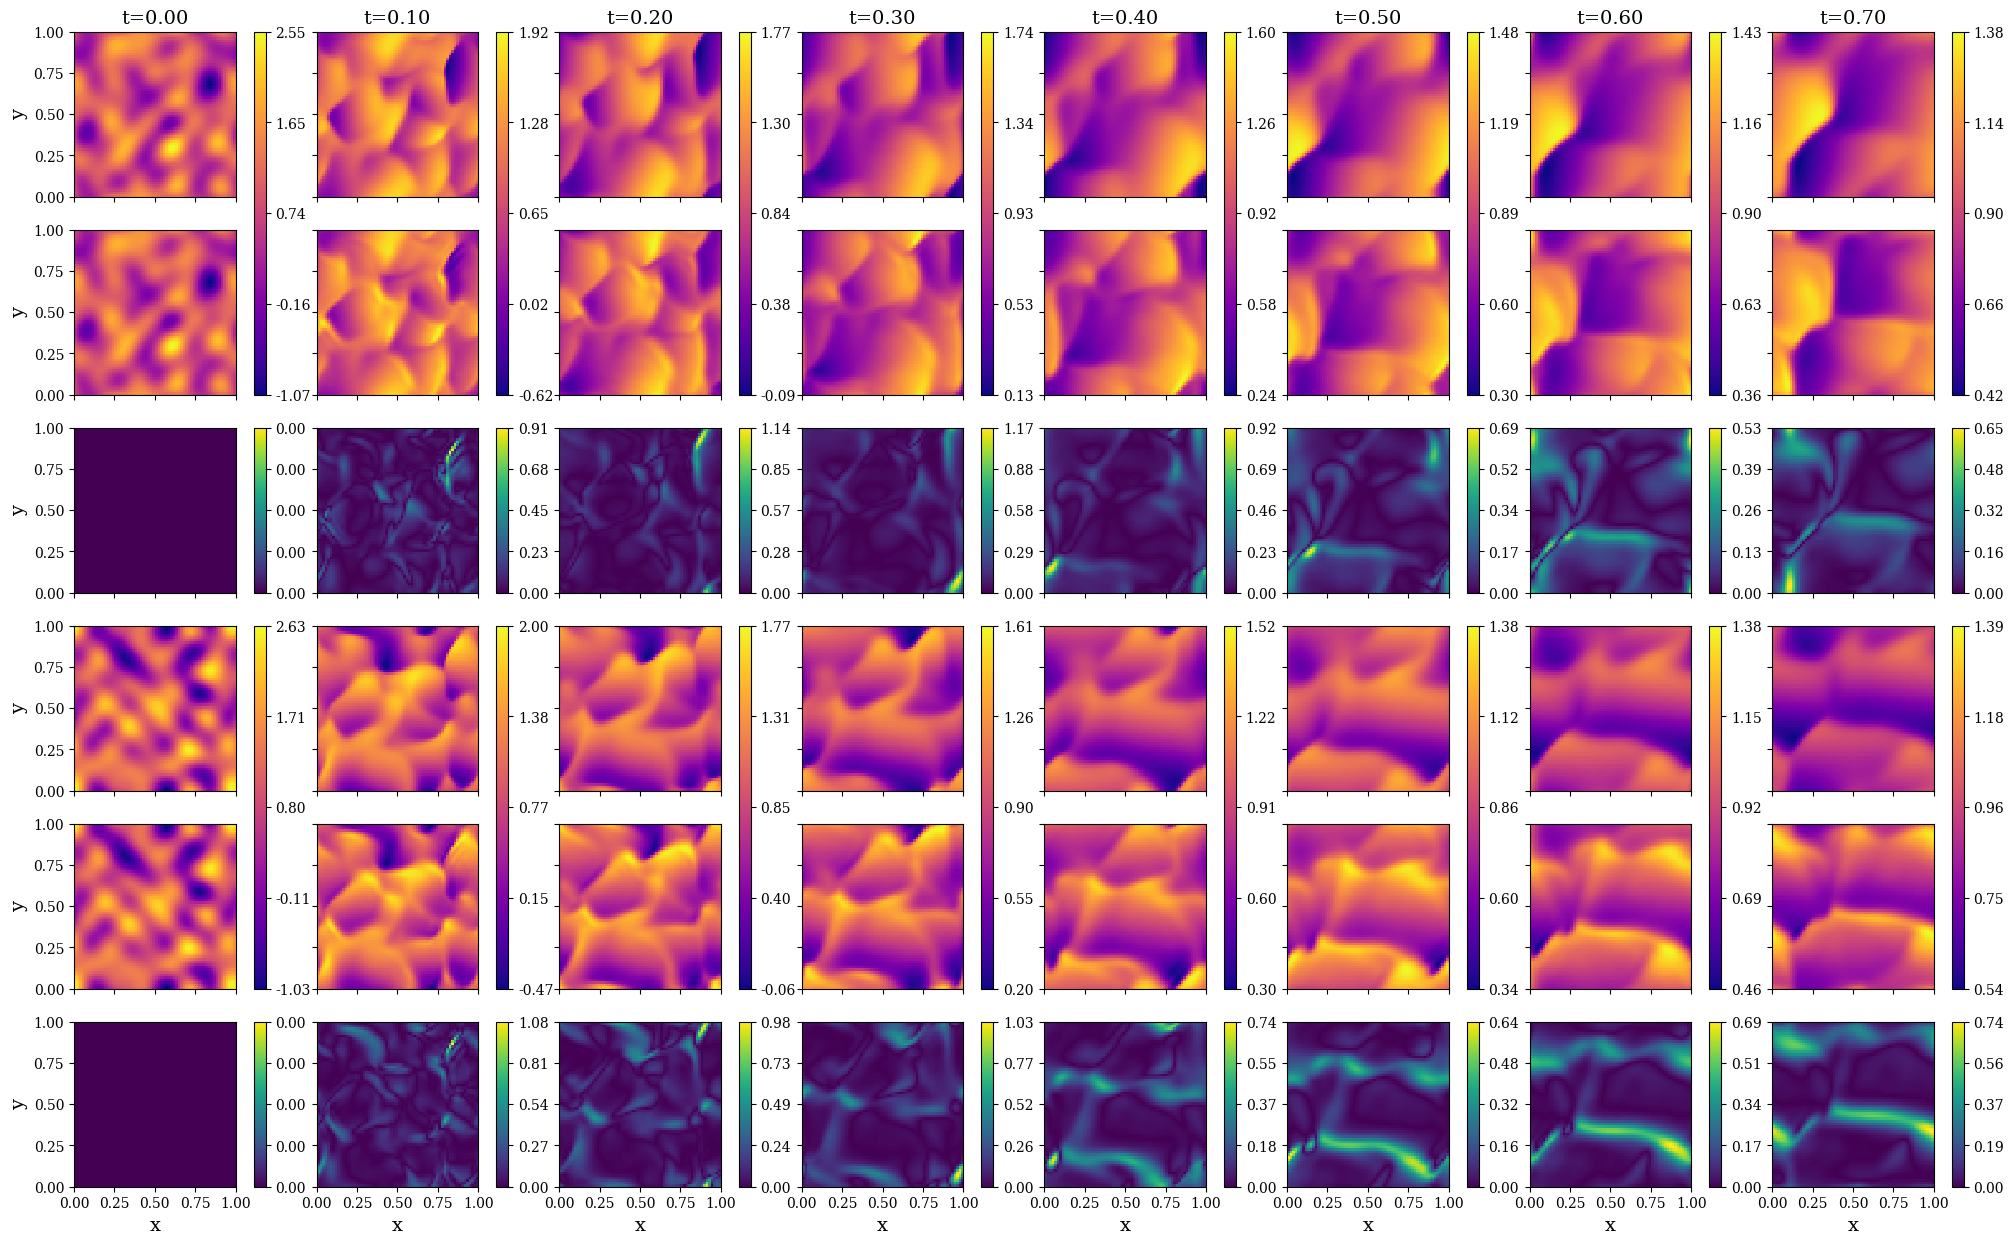
\includegraphics[width=0.8\textwidth]{Fig18.png}
    \caption{AR-DenseED predictions of a 2D coupled Burgers' test case. (Top to bottom) $x$-velocity FEM target solution, $x$-velocity AR-DenseED prediction, $x$-velocity $L_1$ error, $y$-velocity FEM target solution, $y$-velocity AR-DenseED prediction and $y$-velocity $L_1$ error.}
    \label{fig:burgers1D-ARDenseED-1}
\end{figure}

\end{frame}


\begin{frame}
\frametitle{AR-DenseED Deterministic Predictions}
%
\begin{figure}[H]
    \centering
    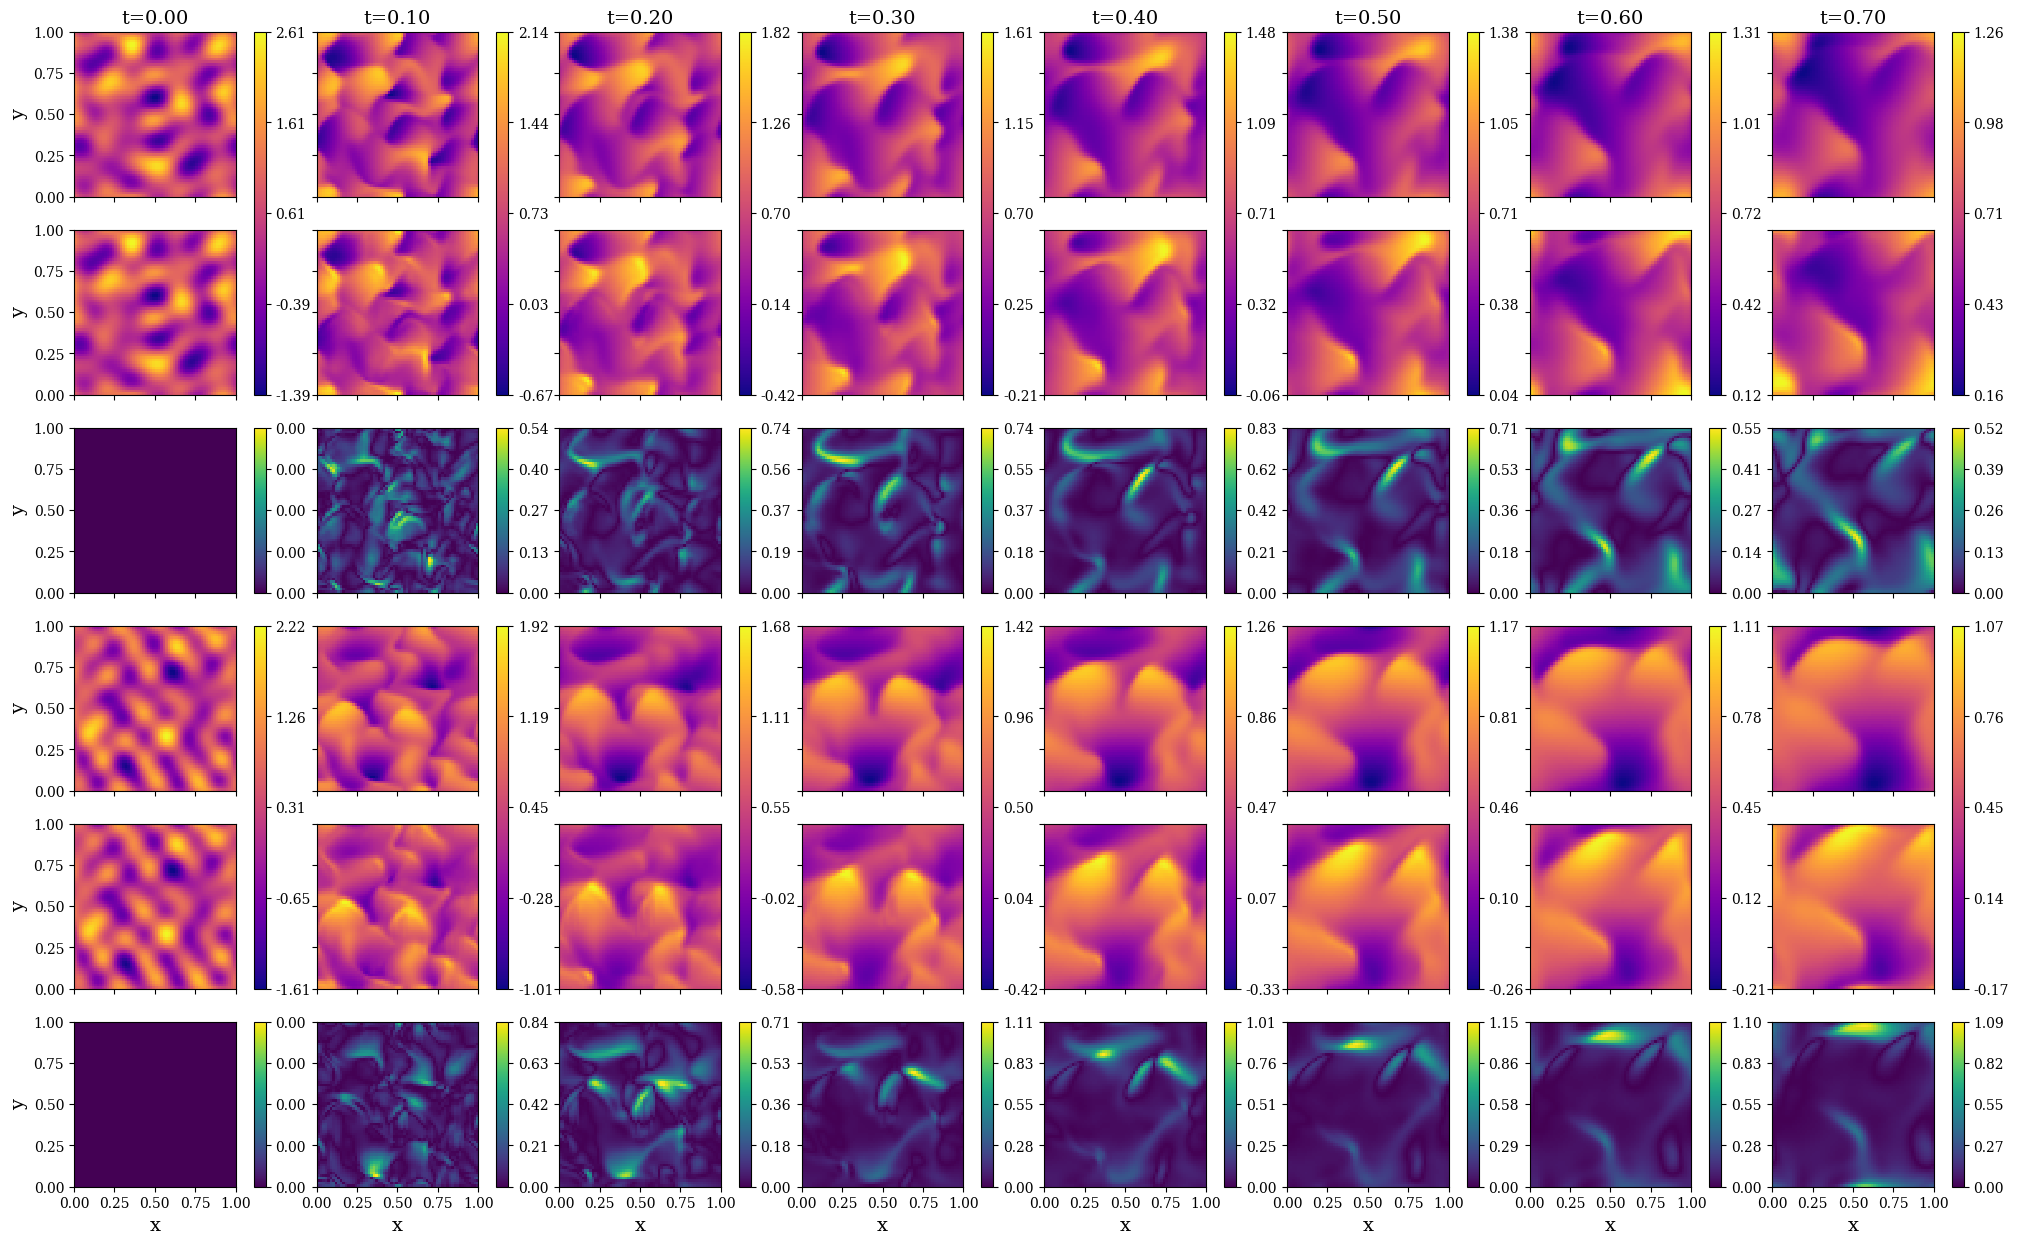
\includegraphics[width=0.8\textwidth]{Fig19.png}
    \caption{AR-DenseED predictions of a 2D coupled Burgers' test case. (Top to bottom) $x$-velocity FEM target solution, $x$-velocity AR-DenseED prediction, $x$-velocity $L_1$ error, $y$-velocity FEM target solution, $y$-velocity AR-DenseED prediction and $y$-velocity $L_1$ error.}
    \label{fig:burgers1D-ARDenseED-2}
\end{figure}
%
\end{frame}

\begin{frame}
\frametitle{AR-DenseED Deterministic Predictions}
%
\begin{figure}[H]
    \centering
    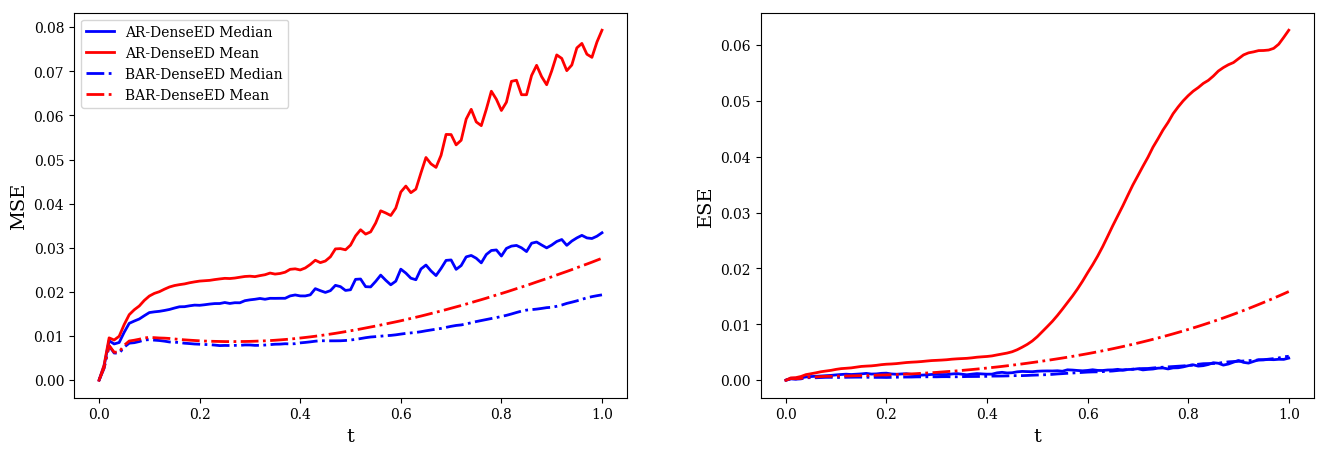
\includegraphics[width=0.9\textwidth]{Fig20.png}
    \caption{(Left to right) The mean square error (MSE) and energy squared error (ESE) as a function of time for a test set of $200$ cases for the 2D coupled Burgers' system.
    The error of BAR-DenseED is calculated using the expected value of the predictive distribution approximating using $30$ samples of the posterior.}
    \label{fig:burgers2D-MSE}
\end{figure}
\end{frame}

\begin{frame}
\frametitle{2D Coupled Burgers' System}
\begin{table}[H]
    \caption{Wall-clock time of finite element simulation and AR-DenseED to simulate $200$ time-steps of the 2D coupled Burgers' system.
    Wall-clock time estimates were obtained by averaging $10$ independent simulation run times.}
    \resizebox{\columnwidth}{!}{
    \begin{tabular}{l|llccc}
                     & \multicolumn{1}{c}{Hardware} & Backend & \multicolumn{1}{c}{$\Delta t$} & \multicolumn{1}{c}{$\Delta x$} & Wall-clock (s) \\ \hline
    Finite Element    & Intel Xeon E5-2680  & Fenics  & $0.005$  & 1/128 & $2955.38$ \\
    Finite Element    & Intel Xeon E5-2680  & Fenics  & $0.005$  & 1/64 & $418.83$ \\
    Finite Element    & Intel Xeon E5-2680  & Fenics  & $0.005$  & 1/32 & $133.65$ \\
    AR-DenseED        & Intel Xeon E5-2680  & PyTorch & $0.005$  & 1/64 & $4.691$  \\
    AR-DenseED        & GeForce GTX 1080 Ti   & PyTorch & $0.005$  & 1/64 & $0.841$
    \end{tabular}}
    \label{tab:burger2d-wallclock}
\end{table}
\end{frame}

\subsection{BAR-DenseED Probabilistic Predictions}

\begin{frame}
\frametitle{BAR-DenseED Probabilistic Predictions}
%
\begin{figure}[H]
    \centering
    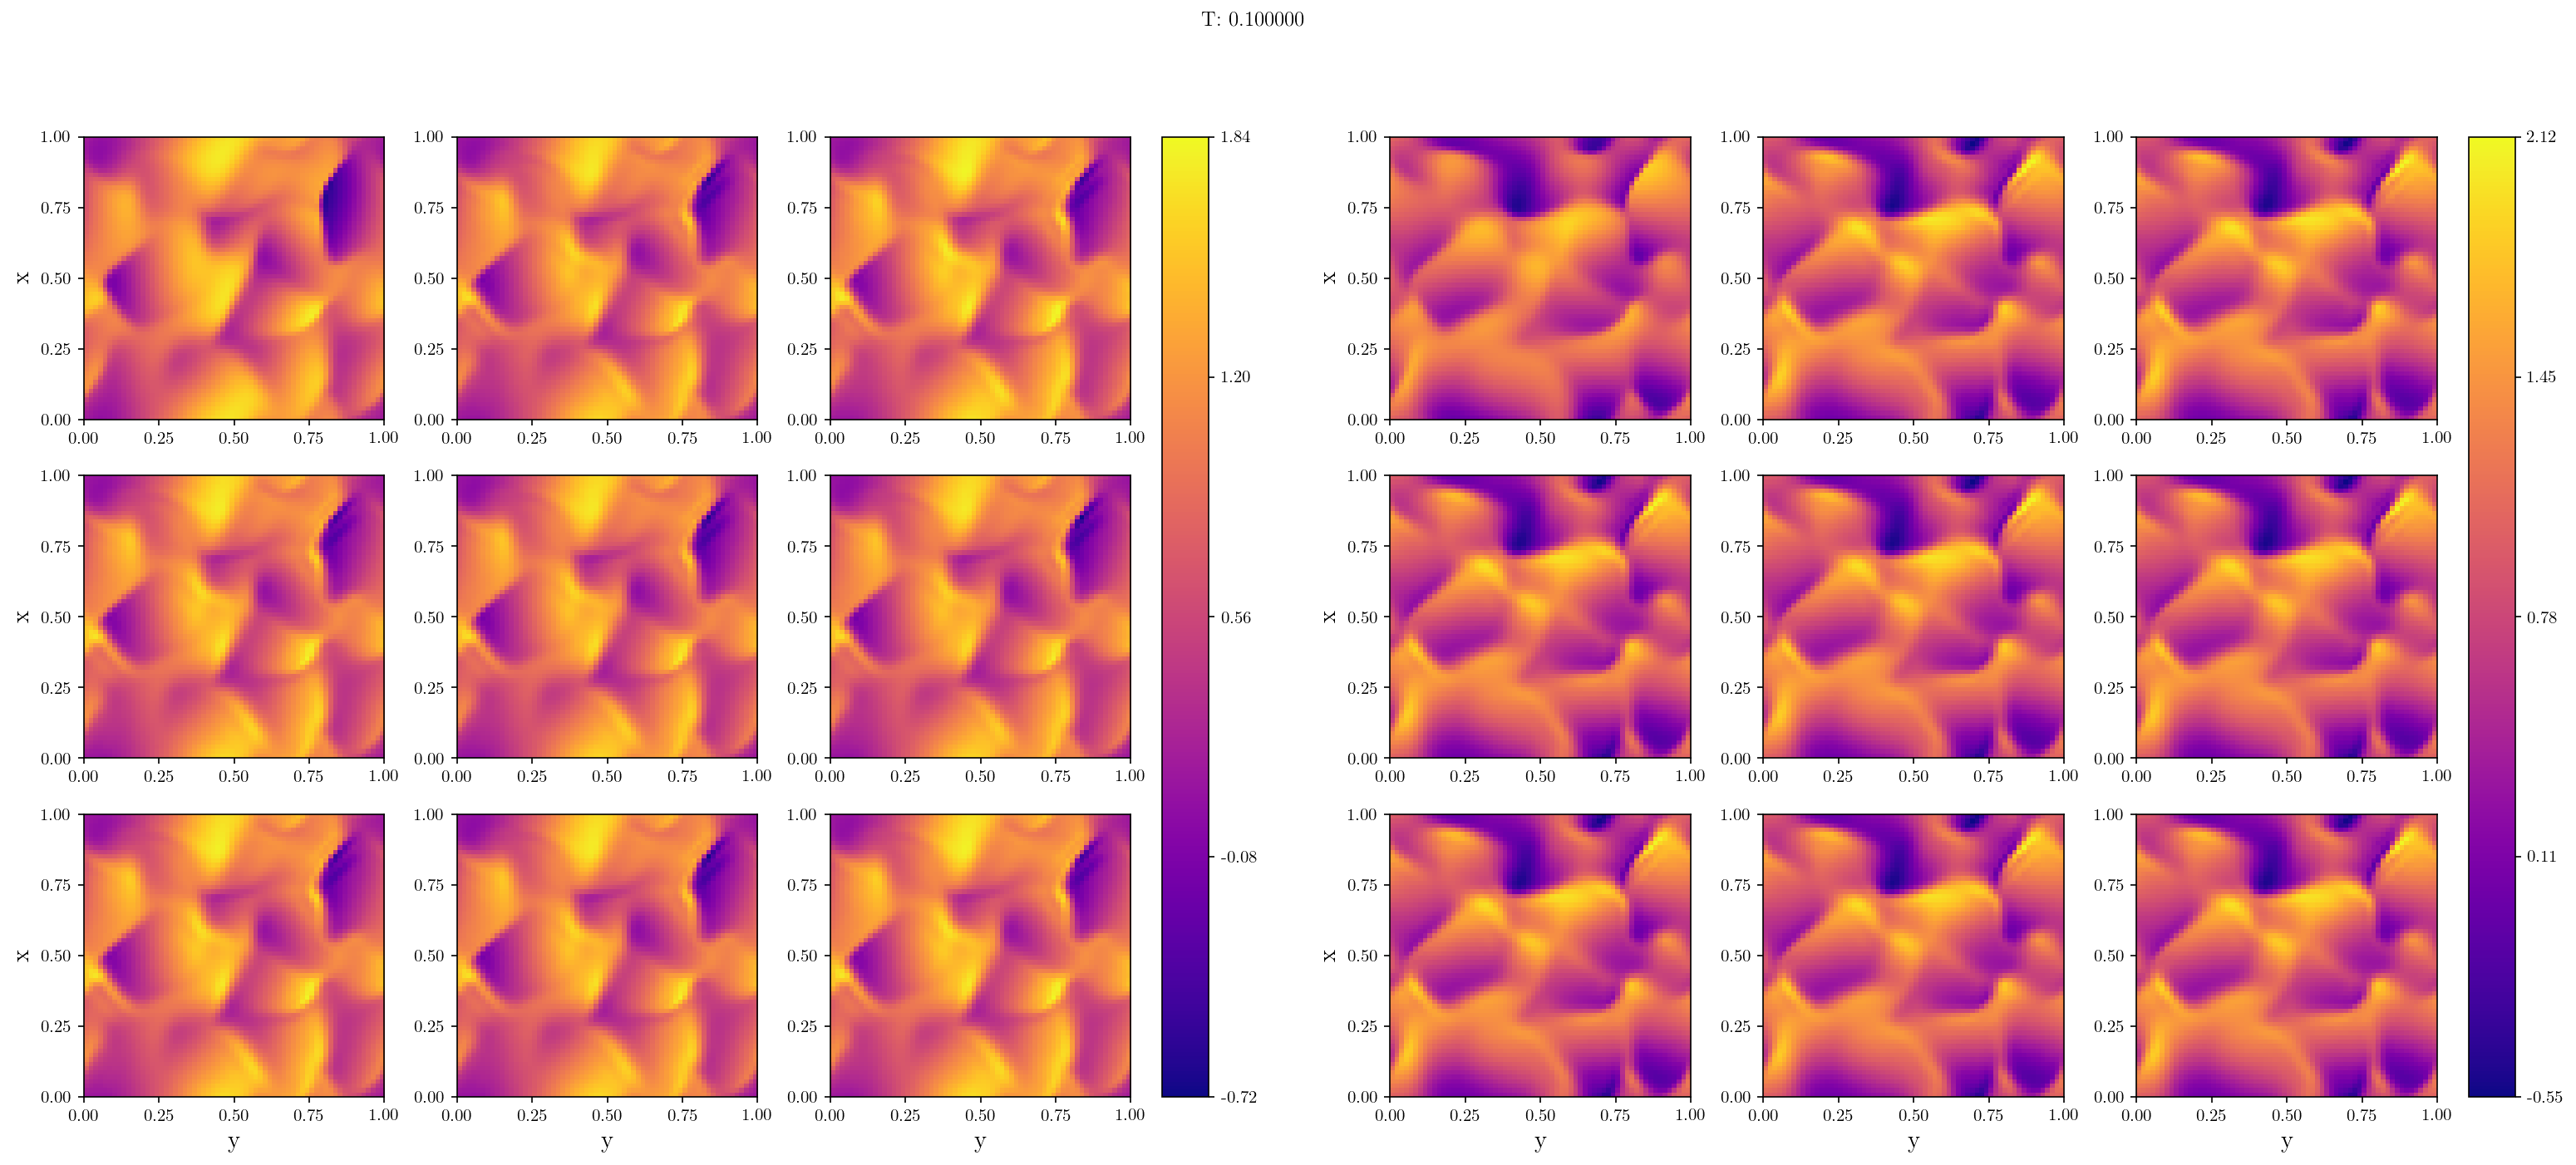
\includegraphics[trim={0 0 0 1cm}, clip, width=0.9\textwidth]{Fig21.png}
    \caption{(Left to right) Samples of the $x$-velocity and $y$-velocity component from the posterior of BAR-DenseED approximated using SWAG at $t=0.1$ for the 2D coupled Burgers' system. The top left in each grid is the simulated result using FEM.} 
    \label{fig:burgers2D-bar-samples-1}
\end{figure}
\end{frame}

\begin{frame}
\frametitle{BAR-DenseED Probabilistic Predictions}
\begin{figure}[H]
    \centering
    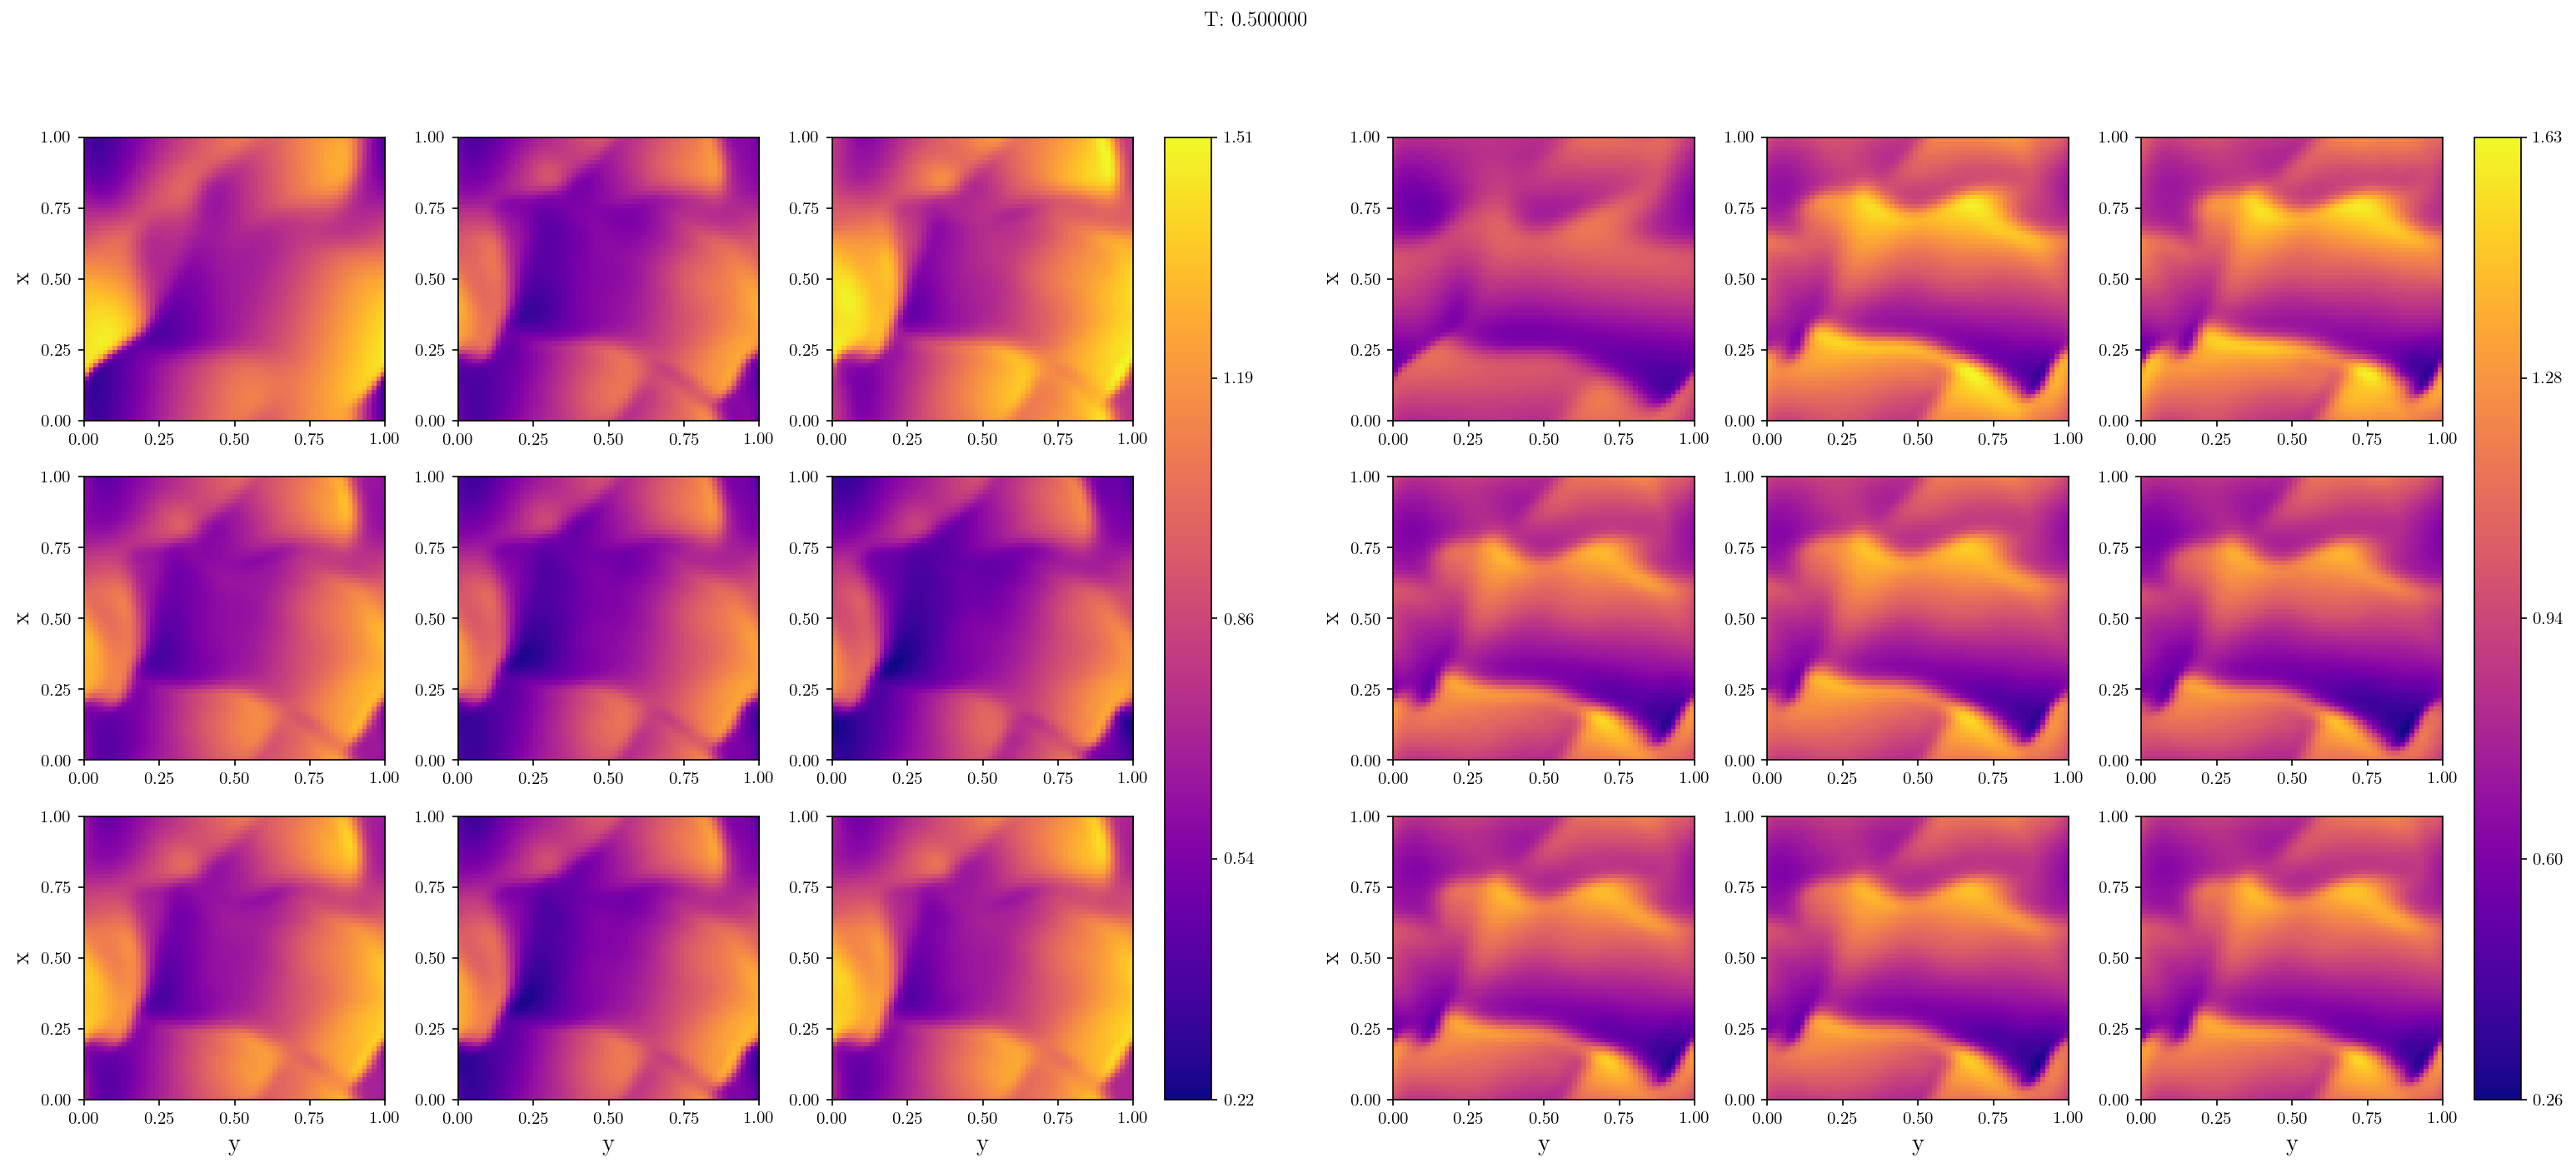
\includegraphics[trim={0 0 0 1cm}, clip, width=0.9\textwidth]{Fig22.png}
    \caption{(Left to right) Samples of the $x$-velocity and $y$-velocity component from the posterior of BAR-DenseED approximated using SWAG at $t=0.5$ for the 2D coupled Burgers' system. The top left in each grid is the simulated result using FEM.} 
    \label{fig:burgers2D-bar-samples-2}
\end{figure}
\end{frame}

\begin{frame}
\frametitle{BAR-DenseED Probabilistic Predictions}
\begin{figure}[H]
    \centering
    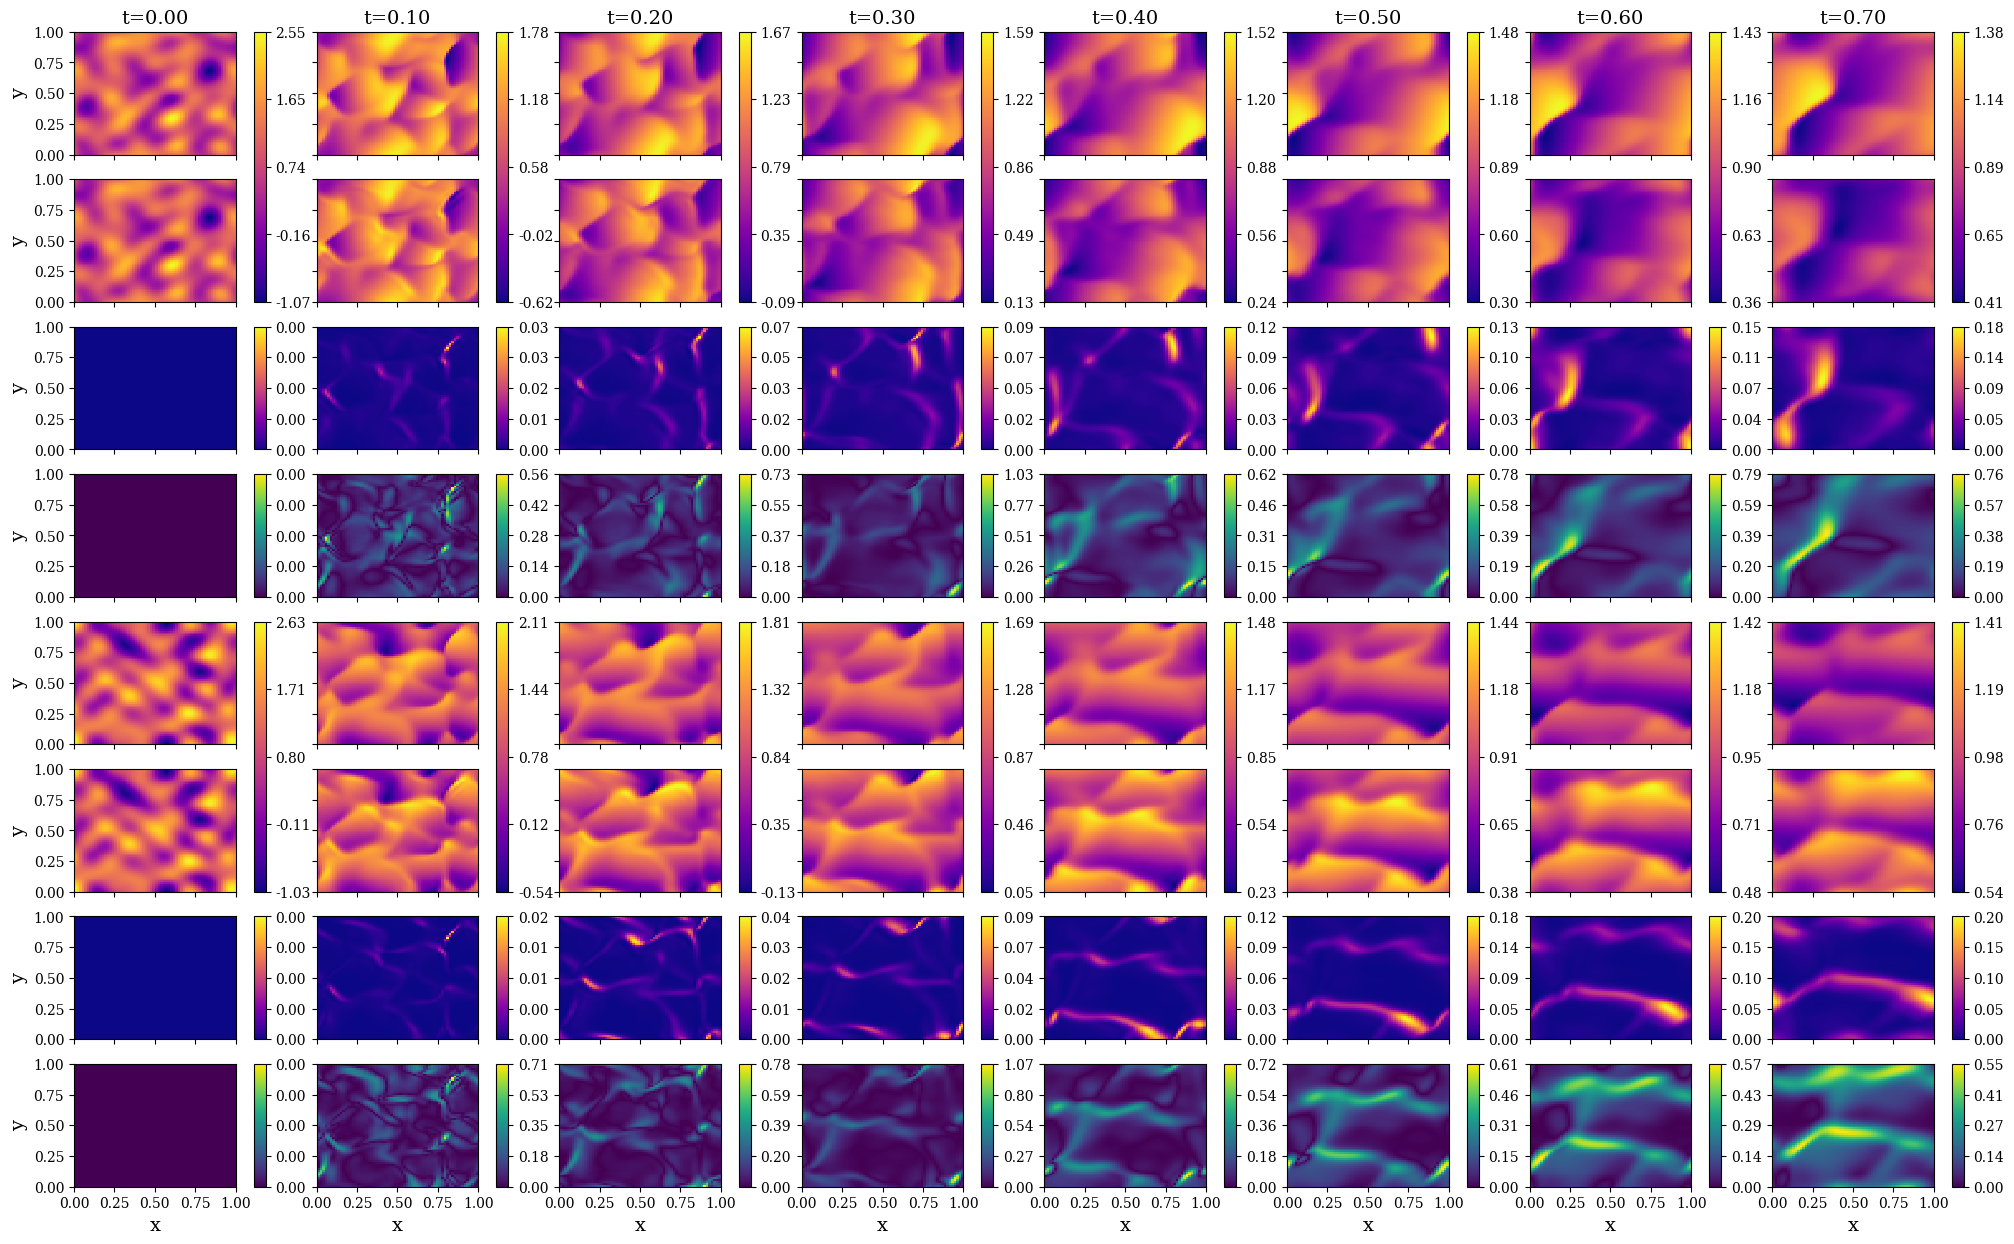
\includegraphics[width=0.85\textwidth]{Fig23.png}
    \caption{BAR-DenseED predictions for a 2D coupled Burgers' test case. (Top to bottom) $x$-velocity FEM target solution, BAR-DenseED expected response, BAR-DenseED variance, $L_1$ error between the target and expected values and similarly followed by the $y$-velocity component. }
    \label{fig:burgers2D-BARDenseED-1}
\end{figure}

\end{frame}

\begin{frame}
\frametitle{BAR-DenseED Probabilistic Predictions}
\begin{figure}[H]
    \centering
    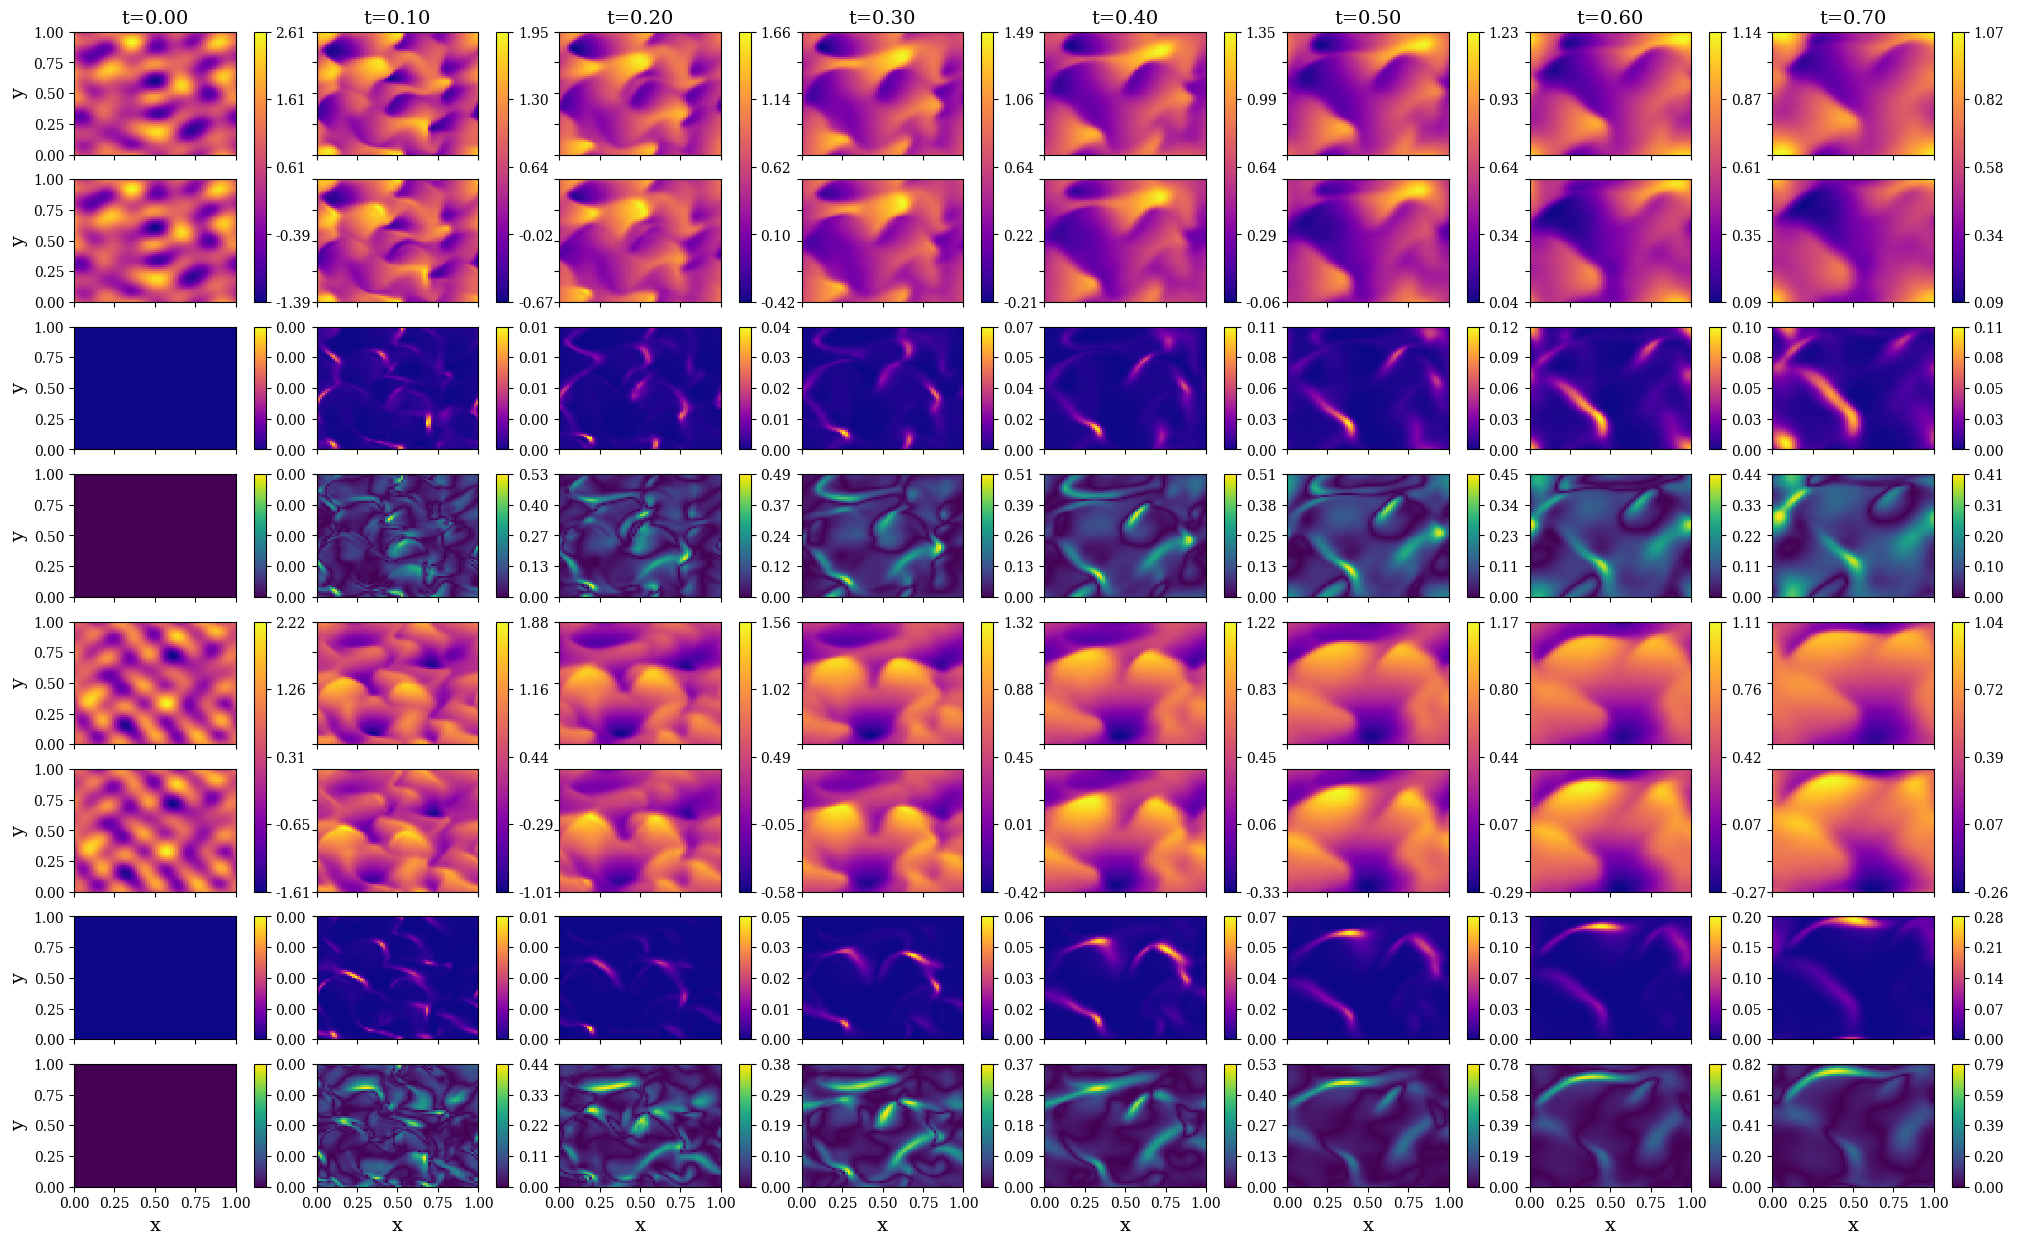
\includegraphics[width=0.77\textwidth]{Fig24.png}
    \caption{BAR-DenseED predictions for a 2D coupled Burgers' test case. (Top to bottom) $x$-velocity FEM target solution, BAR-DenseED expected response, BAR-DenseED variance, $L_1$ error between the target and expected values and similarly followed by the $y$-velocity component.}
    \label{fig:burgers2D-BARDenseED-2}
\end{figure}
\end{frame}

\begin{frame}
\frametitle{BAR-DenseED Probabilistic Predictions}
\begin{figure}[H]
    \centering
    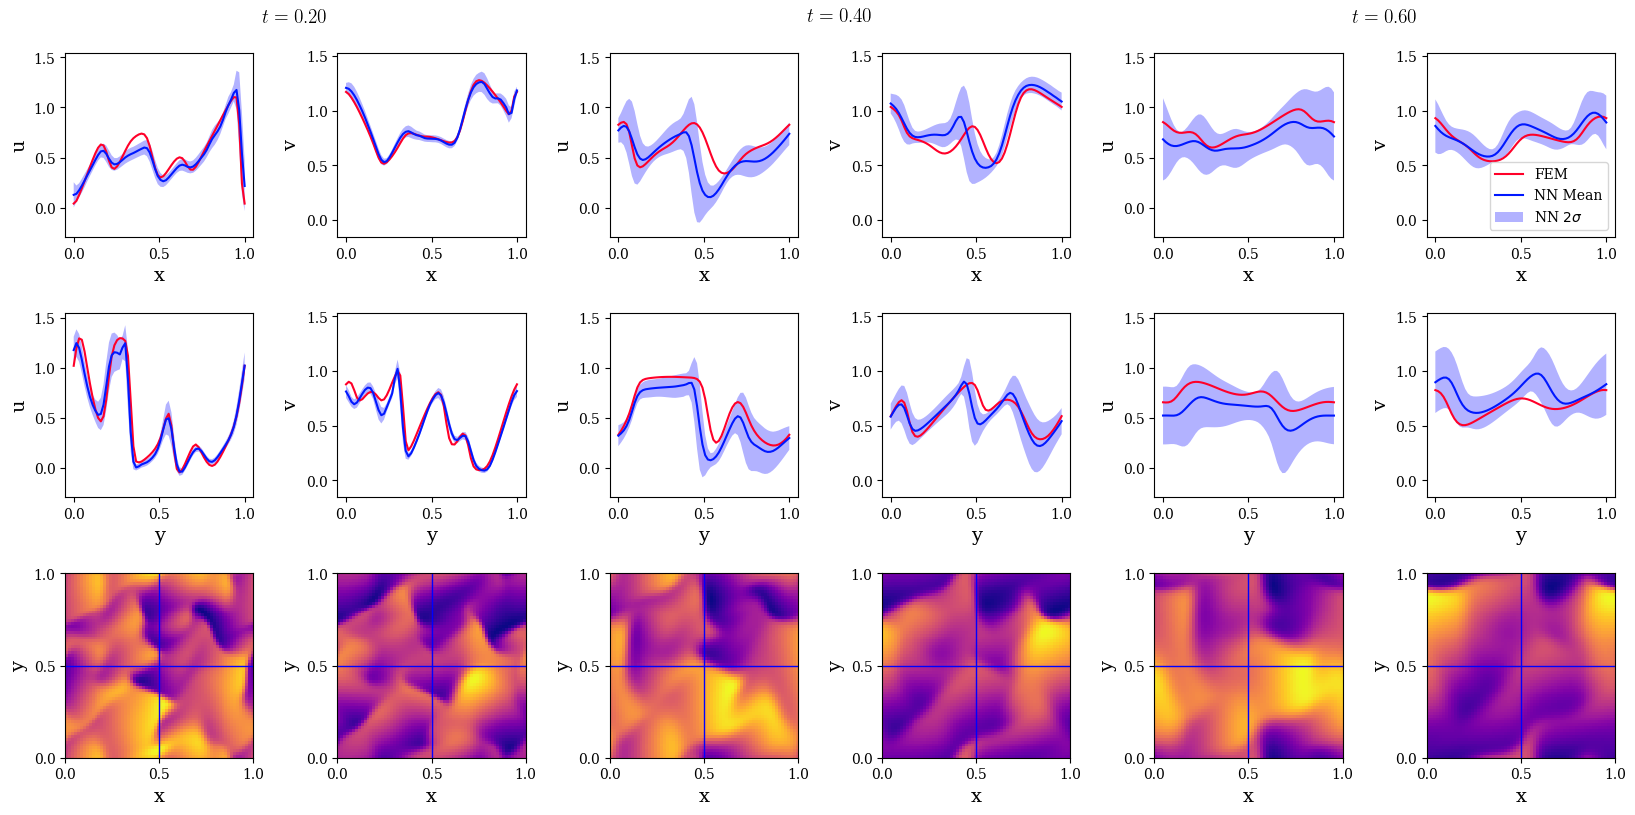
\includegraphics[width=0.8\textwidth]{Fig25.png}
    \caption{Instantaneous profiles of the finite element method (FEM) solver and BAR-DenseED (NN) predictive expectation and standard deviation at three various times of a test case.
    (Top to bottom) Horizontal profile at $y=0.5$, vertical profile at $x=0.5$ and target FEM contour with blue lines to show the profile locations.
    (Left to right) $x$-velocity and $y$-velocity profiles at $t=0.2$, $0.4$ and $0.6$.}
    \label{fig:burgers2D-profiles}
\end{figure}
\end{frame}

\section{Conclusion}

\begin{frame}
\frametitle{Conclusion}
\begin{itemize}
\item{In this work, we have presented a deep auto-regressive convolutional neural network model that can be used to learn and surrogate model the dynamics of transient PDEs.
}
\item{To train this model, physics-constrained deep learning is used where the governing equations of the system of interest are used to formulate a loss function.}
\item{This allows the model to be trained with zero (output) training data.}

\item{Additionally, we proposed a Bayesian probabilistic framework built on top of this deep learning model to allow for uncertainty quantification (including both epistemic and aleatoric uncertainty).}

\end{itemize}
\end{frame}


\begin{frame}
\frametitle{Conclusion}

\begin{itemize}
\item{This model was implemented for three PDE systems: the first is the chaotic Kuramoto-Sivashinsky equation for which the model was used to accurately reproduce physical turbulent statistics.
The second is the 1D Burgers' equation at a low viscosity where the model was able to successfully predict multi-shock wave formation and intersections.}

\item{At last is the 2D coupled Burgers' equations for which the model was able to accurately predict the complex wave dynamics of this system.}

\item{Overall, the proposed model showed exceptional predictive accuracy and was able to successfully extrapolate to predict outside the time-range used when training.}

\item{Although fully connected networks are frequently used to solve PDE systems due to their analytical and mesh-less benefits, the performance of convolutional neural networks for solving and surrogate modeling of PDEs is exceptional.}
\end{itemize}
\end{frame}


\begin{frame}
\frametitle{Limitations}

\begin{itemize}

\item{In this work, we have further shown that convolutional neural networks can be used effectively in physics-constrained learning and build surrogate models that are order of magnitudes faster than state-of-the-art numerical solvers.}

\item{A particular draw-back of convolutional neural networks is the requirement that both spatial and temporal derivatives be discretized, which opens the model up to the challenges that are faced in traditional numerical algorithms such as truncation error, oscillations, convergence criterion and more.}

\item{However, one can also use the deep repository of techniques and tricks developed by the numerical analysis community to address these potential issues.}

\item{This would be an interesting avenue to investigate as one could incorporate methods such as flux limiters or non-oscillatory schemes to yield predictions that have similar numerical benefits.}

\end{itemize}
\end{frame}


\begin{frame}
\frametitle{Future Directions}

\begin{itemize}

\item{One could also consider higher-order derivatives and their impact on accuracy versus training stability.}

\item{The most obvious path to further develop this model is to implement it for more complex and larger systems.}

\item{This could include systems such as the Navier-Stokes equations, coupled transport through porous media, combustion and more.}

\item{However, there are still significant challenges that will need to be addressed.}

\item{The most important is training cost; with any time series problem training a deep learning model becomes exponentially more difficult and more costly.}

\end{itemize}
\end{frame}


\begin{frame}
\frametitle{More Future Directions}

\begin{itemize}

\item{Although our model is able to be trained in a very reasonable amount of time given the complexity of the physical systems modeled as well as the hardware used, improving the training of the model will still be an important area of study.}

\item{This may involve the use of network architectures considered in recent neural language processing literature such as self-attention mechanisms.}

\item{Another potential extension is the incorporation of data and physics-constrained learning to create this hybrid learning framework.}

\item{Specifically for time series, one may not have the system state at every time interval that is desired.}

\item{Physics-constrained learning could be an answer to help bridge this challenge of predicting at fine resolutions with sparse data.}


\end{itemize}
\end{frame}

%------------------------------------------------
%----------------------------------------------------------------------------------------
\bibliography{mybibfile}
\end{document} 
